% documentclass options:
\documentclass[11pt,
  a4paper,
  parskip=half, % This is some extra vertical space between paragraphs, the suggestion is 2cm which is really ugly, so we use what koma script gives us
  % you can also set it to full for even more space. But there is a bad tex style decision: parskip also changes the spacing between listitems such as
  % enumerate and itemize. For this purpose we include the enumitem package and set itemsep=.5em, of course you can change this
  BCOR=10mm, % BCOR is binding correction
  english,
  % if you'd rather have a one sided thesis, add `oneside' to the documentclass
  oneside,
  % ngerman is needed for hyphenation if the thesis contains parts written in German, switch order with english if you write mainly in English.
  % Remember to change order in the babel package (below) as well.
  % Last language is the preferred one.
  english]{scrbook}
\usepackage[english]{babel} % If you write mainly in English change order to ngerman, english. Also change that in the documentclass options above.
% Include of titling must happen before \title etc.
% that's why it's not in setup.tex
\usepackage{titling}
\title{Porting the rRNA-prediction part of the MGnify amplicon analysis pipeline to Galaxy}
\author{Rand Zoabi}

% Change to your first examiner
% The ~ enables non sentence spacing after a period
\newcommand{\firstexaminer}{Prof.~Dr. Rolf Backofen}
% Change to your adivers
\newcommand{\advisers}{Dr. Paul Zierep}
% include all packages and define commands in setup.tex

%------------------------------------------------------------------------------
%       package includes
%------------------------------------------------------------------------------
% font encoding is set up for pdflatex, for other environments see
% http://tex.stackexchange.com/questions/44694/fontenc-vs-inputenc
\usepackage[T1]{fontenc}  % 8-bit fonts, improves handling of hyphenations
\usepackage[utf8]{inputenc}
% provides `old' commands for table of contents. Eases the ability to switch
% between book and scrbook
\usepackage{scrhack}

\usepackage{csquotes}

% ------------------- layout, default -------------------
% adjust the style of float's captions, separated from text to improve readability
\usepackage[labelfont=bf, labelsep=colon, format=hang, textfont=singlespacing]{caption}
% With format = hang your caption will look like this:
% Figure 1: Lorem ipsum dolor sit amet,
%           consectetuer adipiscing elit.
%           Ut purus elit, vestibulum
% If you instead want
% Figure 1: Lorem ipsum dolor sit amet,
% consectetuer adipiscing elit. Ut purus
% elit, vestibulum
% change to format=plain
\usepackage{chngcntr}  % continuous numbering of figures/tables over chapters
\counterwithout{equation}{chapter}
\counterwithout{figure}{chapter}
\counterwithout{table}{chapter}

% Uncomment the following line if you switch from scrbook to book
% and comment the setkomafont line
%\usepackage{titlesec}  % remove "Chapter" from the chapter title
%\titleformat{\chapter}[hang]{\bfseries\huge}{\thechapter}{2pc}{\huge}
\setkomafont{chapter}{\normalfont\bfseries\huge}

\usepackage{setspace}  % Line spacing
\onehalfspacing
% \doublespacing  % uncomment for double spacing, e.g. for annotations in correction

% ------------------- functional, default-------------------
\usepackage[dvipsnames]{xcolor}  % more colors
\usepackage{array}  % custom format per column in table - needed on the title page
% \usepackage{graphicx}  % include graphics
\usepackage{graphicx,verbatimbox,caption,stackengine}\usepackage{subfig}  % divide figure, e.g. 1(a), 1(b)...
\usepackage{amsmath}  % |
\usepackage{amsthm}   % | math, bmatrix etc
\usepackage{amsfonts} % |
\usepackage{calc}  % calculate within LaTeX
\usepackage[unicode=true,bookmarks=true,bookmarksnumbered=true,
    bookmarksopen=true,bookmarksopenlevel=1,breaklinks=false,
    pdfborder={0 0 0},backref=false,colorlinks=false]{hyperref}
\usepackage{etoolbox} % if-else commands


%==========================================
% You might not need the following packages, I only included them as they
% are needed for the example floats
% ------------------- functional, custom -------------------
\usepackage{algorithm,algpseudocode}
\usepackage{bm}  % bold greek variables (boldmath)
\usepackage{tikz}
\usetikzlibrary{positioning}  % use: above left of, etc

% Required for the ToDo list.
\usepackage{ifthen}

% Improves general appearance of the text
\usepackage[protrusion=true,expansion=true, kerning]{microtype}
\usepackage{enumitem}
% Nicer font for pdf rendering.
\usepackage{lmodern}

% For nicer looking tables.
\usepackage{booktabs}

% You don't need this, just for demonstration of a longer caption.
\usepackage{lipsum}


\usepackage{setspace}

%------------------------------------------------------------------------------
%       (re)new commands / settings
%------------------------------------------------------------------------------
% ----------------- referencing ----------------
\newcommand{\secref}[1]{Section~\ref{#1}}
\newcommand{\chapref}[1]{Chapter~\ref{#1}}
\renewcommand{\eqref}[1]{Equation~(\ref{#1})}
\newcommand{\figref}[1]{Figure~\ref{#1}}
\newcommand{\tabref}[1]{Table~\ref{#1}}

% ------------------- colors -------------------
\definecolor{darkgreen}{rgb}{0.0, 0.5, 0.0}
% Colors of the Albert Ludwigs University as in
% https://www.zuv.uni-freiburg.de/service/cd/cd-manual/farbwelt
\definecolor{UniBlue}{RGB}{0, 74, 153}
\definecolor{UniRed}{RGB}{193, 0, 42}
\definecolor{UniGrey}{RGB}{154, 155, 156}


% ------------------- layout -------------------
% prevents floating objects from being placed ahead of their section
\let\mySection\section\renewcommand{\section}{\suppressfloats[t]\mySection}
\let\mySubSection\subsection\renewcommand{\subsection}{\suppressfloats[t]\mySubSection}



% ------------------- math formatting commands -------------------
% define vectors to be bold instead of using an arrow
\renewcommand{\vec}[1]{\mathbf{#1}}
\newcommand{\mat}[1]{\mathbf{#1}}
% tag equation with name
\newcommand{\eqname}[1]{\tag*{#1}}

\usepackage{pmboxdraw}

% ------------------- pdf settings -------------------
% ADAPT THIS
\hypersetup{pdftitle={\thetitle},
    pdfauthor={\theauthor},
    pdfsubject={Undergraduate thesis at the Albert Ludwig University of Freiburg},
    pdfkeywords={forensic},
    pdfpagelayout=OneColumn, pdfnewwindow=true, pdfstartview=XYZ, plainpages=false}


%==========================================
% You might not need the following commands, I only included them as they
% are needed for the example floats

% ------------------- Tikz styles -------------------
\tikzset{>=latex}  % arrow style


% ------------------- algorithm ---------------------
% Command to align comments in algorithm
\newcommand{\alignedComment}[1]{\Comment{\parbox[t]{.35\linewidth}{#1}}}
% define a foreach command in algorithms
\algnewcommand\algorithmicforeach{\textbf{foreach}}
\algdef{S}[FOR]{ForEach}[1]{\algorithmicforeach\ #1\ \algorithmicdo}

% line spacing should be 1.5
\renewcommand{\baselinestretch}{1.5}

% set distance between items in a list, for more details see the
% enumitem package: https://www.ctan.org/pkg/enumitem
\setlist{itemsep=.5em}

% use ra in your tables to increase the space between rows
% 1.3 should be fine
\newcommand{\ra}[1]{\renewcommand{\arraystretch}{#1}}

% ToDo counters
\usepackage{ifthen} %für whiledo-Schleife
\newcounter{todos}
\setcounter{todos}{0}
\newcounter{extends}
\setcounter{extends}{0}
\newcounter{drafts}
\setcounter{drafts}{0}

% ------------------- marker commands -------------------
% ToDo command
\newcommand{\todo}[1]{\textbf{\textcolor{red}{TODO: #1}}\refstepcounter{todos}\label{todo \thetodos}}
\newcommand{\extend}[1]{\textbf{\textcolor{darkgreen}{EXTEND: #1}} \refstepcounter{extends} \label{extend \theextends}}
% Lighter color to note down quick drafts
\newcommand{\draft}[1]{\textbf{\textcolor{NavyBlue}{DRAFT: #1}}\refstepcounter{drafts}\label{draft \thedrafts}}

% microtype with lmodern, see https://tex.stackexchange.com/questions/75305/microtype-warning-with-lmodern-package-and-koma-script
%\DeclareMicrotypeAlias{lmss}{cmr}

\usepackage[style=numeric,
	    citestyle=numeric,
	    backend=biber,
	    sorting=none]{biblatex}

\usepackage[acronym,nomain,nonumberlist]{glossaries}
\makeglossaries
%\ExecuteBibliographyOptions{
%sorting=nyt, %Sortierung Autor, Titel, Jahr
%bibwarn=true, %Probleme mit den Daten, die Backend betreffen anzeigen
%isbn=true, %keine isbn anzeigen
%url=true % url anzeigen
%}

\addbibresource{bib/references.bib}

% Comment to show all figures
% \usepackage[figuresonly,nolists,nomarkers]{endfloat}
% \renewcommand{\processdelayedfloats}{}

\usepackage{cleveref}
\usepackage{url}
\usepackage{pdflscape}
\usepackage{graphicx}
\usepackage{geometry}
\usepackage{fancyhdr}
\usepackage{lscape}


\begin{document}
\pagestyle{empty} % no header and no page number
% disable hyper links to remove warning "destination with same identifier"
% this means within this section nothing can be referenced with a hyperlink
\hypersetup{pageanchor=false}

% enable/disable, depending on your chosen language
\begin{titlepage}
	\begin{center}

		\newcommand{\HorizontalLine}{\rule{\linewidth}{0.3mm}}

		{\Large Bachelor Thesis}\\[1.3cm]


		% _____________________________________________________________________________
		\HorizontalLine \\[0.4cm]
		% Write yourtitle in a fancy way like this if you want to customize it, otherwise simply let tex do it for you
		% \begin{spacing}{3}
		%     {\huge \bfseries Der Lange, Lange } \\
		%     {\huge \bfseries Lange Lange} \\
		%     {\huge \bfseries Titel}\\
		% \end{spacing}
		{ \huge \bfseries \thetitle }
		\HorizontalLine \\[2cm]
		% _____________________________________________________________________________


		{\Huge \theauthor} \\[2.6cm]


		\begin{tabular}[hc]{>{\huge}l >{\huge}l}
			Examiner: & \firstexaminer \\[0.3cm]
			Advisor:  & \advisers      \\[2.6cm]
		\end{tabular}
		\vfill  % move the following text to the bottom

		\Large {
			Albert-Ludwigs-Universität Freiburg\\
			Faculty of Engineering\\
            Department of Computer Science\\
			Chair of Bioinformatics\\[0.7cm]

			05. Oct 2023
			\\
		}
	\end{center}
\end{titlepage}

\thispagestyle{empty}
% title page back
\ \vfill \ \\  % at least one space required before vfill
\
\textbf{Writing Period}            \smallskip{} \\
05.\,07.\,2023 -- 05.\,10.\,2023   	 \bigskip{} \\
\
\textbf{Examiner}                  \smallskip{} \\
\firstexaminer                      \bigskip{} \\
\
\textbf{Advisor}                  \smallskip{} \\
\advisers

\pagestyle{plain} % remove chapter name from top, page number at the bottom
% use \pagestyle{headings} for having the chapter on top of the pages
% if you wang a more fancy header use \usepackage[automark,headsepline]{scrlayer-scrpage}
% and read about it in the KOMA script documentation, https://www.ctan.org/pkg/koma-script
\frontmatter  % roman page numbers
\chapter*{Declaration}
I hereby declare, that I am the sole author and composer of my thesis and that no
other sources or learning aids, other than those listed, have been used. Furthermore,
I declare that I have acknowledged the work of others by providing detailed
references of said work.
I also hereby declare that my thesis has not been prepared for another examination
or assignment, either in its entirety or excerpts thereof.
\\[3\normalbaselineskip]
\begin{tabular}{p{\textwidth/2} l}
  \rule{\textwidth/3}{0.4pt}  & \rule{\textwidth/3}{0.4pt} \\
  Place, date                  & Signature
\end{tabular}
\chapter*{Acknowledgements}
First and foremost, I express my gratitude to Prof. Dr. Rolf Backofen, who agreed to review this work and gave me the opportunity to work on this interesting topic.\\
Special thanks are owed to Dr. Paul Zierep for the best supervision one could wish for. Thank you for always being open to my questions, for your invaluable advice, and for keeping me motivated throughout this journey. Working with you was enriching and valuable. I appreciate your dedicated efforts.\\
I would also like to express my gratitude to Dr. Paul Zierep, Dr. Björn Grüning, and Dr. Matthias Bernt for reviewing my tool wrapper pull requests on GitHub and for their improvement suggestions.\\
I extend my appreciation to Dr. Alexandre Almeida for addressing my questions regarding the samples from his study.\\
A special acknowledgment goes also to the MGnify team for being open for questions regarding the pipeline, and it tools, which contributed to this thesis.\\
Lastly, I would like to thank my family and friends for their support in various ways throughout the writing of this thesis.

\chapter*{Abstract}

Metagenomic sequencing is a powerful method used to uncover and characterize microbial communities by analyzing genetic material from environmental samples. This thesis benchmarks the performance of Kraken2, Bracken, MetaPhlAn, and mOTUs using the CAMI challenge dataset as a gold standard within the Galaxy framework.
The benchmarking process compared the taxonomic profiling outputs of these tools against the CAMI gold standard using Cami Opal for detailed analysis. Metrics such as taxonomic profiling accuracy, computational efficiency, and memory usage were assessed. Kraken2 and Bracken provided high accuracy, while MetaPhlAn and mOTUs effectively profiled microbial communities using marker genes.
Integrating these tools into Galaxy enhances their utility for metagenomic research by providing a reproducible and customizable analysis environment. The study highlights the strengths and limitations of each tool, offering valuable insights for selecting the appropriate pipeline for specific research needs.
The availability of these tools within Galaxy offers several advantages for the metagenomics research community, including interoperability, reproducibility, and ease of use, facilitating advanced downstream analyses such as machine learning and differential abundance analysis.

\vspace{1cm}

\textbf{Deutsche Version:}

\vspace{0.5cm}

Metagenomisches Sequenzieren ist eine leistungsstarke Methode zur Entdeckung und Charakterisierung mikrobieller Gemeinschaften durch die Analyse genetischen Materials aus Umweltproben. Diese Arbeit vergleicht die Leistung von Kraken2, Bracken, MetaPhlAn und mOTUs anhand des CAMI-Challenge-Datensatzes als Goldstandard im Galaxy-Framework.
Der Benchmarking-Prozess verglich die taxonomischen Profilierungsausgaben dieser Werkzeuge mit dem CAMI-Goldstandard unter Verwendung von Cami Opal für eine detaillierte Analyse. Metriken wie die Genauigkeit der taxonomischen Profilierung, die Recheneffizienz und die Speichernutzung wurden bewertet. Kraken2 und Bracken boten eine hohe Genauigkeit, während MetaPhlAn und mOTUs effektiv mikrobiellen Gemeinschaften mit Markergenen profilierten.
Die Integration dieser Werkzeuge in Galaxy erhöht deren Nutzen für die metagenomische Forschung durch eine reproduzierbare und anpassbare Analyseumgebung. Die Studie hebt die Stärken und Schwächen jedes Werkzeugs hervor und bietet wertvolle Einblicke in die Auswahl der geeigneten Pipeline für spezifische Forschungsanforderungen.
Die Verfügbarkeit dieser Werkzeuge im Galaxy-Framework bietet der Metagenomik-Forschungsgemeinschaft mehrere Vorteile, darunter Interoperabilität, Reproduzierbarkeit und Benutzerfreundlichkeit, und erleichtert fortschrittliche nachgelagerte Analysen wie maschinelles Lernen und Differenzanalyse der Abundanz.
\tableofcontents
% \listoffigures
% \listoftables
% \listofalgorithms
\hypersetup{pageanchor=true}  % re-enable hyperlinking

\newacronym{cami}{CAMI}{The Critical Assessment of Metagenome Interpretation}
\newacronym{otu}{OTU}{Operational Taxonomic Unit}
\newacronym{ssu}{SSU}{Small Subunits}
\newacronym{lsu}{LSU}{Large Subunits}
\newacronym{rrna}{rRNA}{Ribosomal Ribonucleic Acid}
\newacronym{cwl}{CWL}{Common Workflow Language}
\newacronym{cm}{CM}{Covariance Model}


\glsaddall
\printglossary[type=\acronymtype,title=Acronyms]

\mainmatter  % Arabic page numbers
\chapter{Introduction}\label{chap:Introduction}

Amplicon sequencing is a research method, designed to uncover the taxonomic composition of microbial communities. Ribosomal ribonucleic acid (rRNA) or ribosomal deoxyribonucleic acid (rDNA) are sequenced by targeting specific genes such as 16S for bacteria and archaea, 18S for eukaryota, or internal transcribed spacers (ITS) regions for fungi. Amplicon sequencing, compared to whole genome sequencing, is cost-effective and consumes less time~\cite{fricker_what_2019}. Amplicon sequencing is employed in a broad range of fields such as cancer research~\cite{guerrero-preston_16s_2016}, forensics~\cite{zhang_application_2023}, and food safety~\cite{mira_miralles_high-throughput_2019}.\\
Various pipelines/tools can be used in conjunction of different databases for amplicon analysis. Given the absence of a definitive singular approach, several studies were conducted (mentioned in \Cref{chap:State_of_the_art}) in recent years. These studies compared time cost, memory usage, and accuracy, across the spectrum of tools when paired with the different databases.

\section{MGnify}\label{sec:MGnify-intro}

MGnify offers a free-to-use service for the analysis and archiving of microbiome data.
The pipelines and used tools are open source (GitHub~\cite{noauthor_mgnify_nodate-22}). Each workflow is comprehensively documented using the Common Workflow Language (CWL)~\cite{language_cwl_home_nodate}, enhancing the reproducibility of the pipelines~\cite{mitchell_mgnify_2020}. Version 5.0 of MGnify offers three analysis pipelines associated with distinct input types: amplicon data, raw metagenomic reads, and assembly~\cite{noauthor_mgnify_nodate-25}. At the time of writing this thesis, MGnify had analyzed 356,039 amplicon analyses, 28,873 assemblies, and 33,827 metagenomic analyses~\cite{noauthor_mgnify_nodate-23}.
\section{Galaxy project}\label{sec:Galaxy-intro}
Galaxy is a free-to-use web-based platform for scientific computing. It offers a user-friendly interface for running tools/workflows on large data-sets, the workflow manager allows users to create new workflows, but also to import and edit already existing ones~\cite{the_galaxy_community_galaxy_2022}. Galaxy offers a wide range of tutorials covering various scientific and technical topics, by the time of writing 321 contributors have contributed their work on 360 tutorials covering 37 topics such as metagenomics, transcriptomics, variant analysis etc.~\cite{noauthor_galaxy_0000}.

\section{Aim of this thesis}\label{aim_of_thesis}
Although MGnify is documented using CWL, the pipeline is technically difficult to execute and requires vast computational resources. Therefore, individual users can only use the analysis service provided by MGnify. To facilitate individual execution of MGnify's analysis pipeline and concurrently offer computational resources, this thesis aims to investigate the feasibility to port the MGnify pipelines v5.0 into the Galaxy framework. The availability on Galaxy will offer several additional advantages such as interoperability, reproducibility, shareability, integration with MGnify Jupyter Notebooks, exchange of specific tools (e.g. for quality control), as well as downstream analysis using machine learning and differential abundance analysis .\\
Due to the limited time scope of this bachelor thesis, the efforts had to be concentrated on a single pipeline. The decision was made to port the amplicon pipeline. Given the commonality of the rRNA-prediction subworkflow across all three pipelines~\cite{mgnify_mgnify_2023}, it was selected as the component for integration. The availability of quality-checked reads in MGnify, which serve as an input to the rRNA-prediction subworkflow, offered the opportunity to bypass the quality control subworkflow and facilitate benchmarking of the ported version of the rRNA-prediction subworkflow against its original counterpart. The ported pipeline was benchmarked using beta diversity metrics to measure the dissimilarity values between the taxonomic abundance outputs for different taxonomic ranks.\\
Building upon prior studies (\Cref{sec:Kraken}) that found Kraken v2 to be superior in some cases as compared to purely amplicon based pipelines, the ported subworkflow was furthermore compared to Kraken v2.
\chapter{State of the art}\label{chap:State_of_the_art}

\section{MGnify amplicon pipeline}\label{sec:MGnify}
Version 5.0 of the amplicon pipeline was enhanced by incorporating classification of fungi based on the internal transcribed spacer (ITS) regions, in addition to the small subunits (SSU) and large subunits (LSU) based classifications that were already present in the previous version~\cite{mitchell_mgnify_2020}. If the data consists of paired-end reads, the amplicon pipeline initiates by merging the reads using SeqPrep v1.2, as shown in the complete amplicon flowchart in \Cref{fig:amplicon-pipline}. Subsequently, the merged reads undergo quality control, using Trimmomatic v0.36 to trim low-quality sequencing regions. Following quality control, the rRNA-prediction subworkflow is executed. The subworkflow comprises a search against Rfam v13.0 SSU and LSU models utilizing cmsearch v1.1.2. Furthermore, MAPseq v1.2.3, in conjunction with the SILVA v132 database, conducts taxonomic classification. The outputs consist of abundance tables visualized using Krona v2.7.1 as pie charts. The charts and outputs of the pipeline are accessible via the MGnify website~\cite{noauthor_mgnify_nodate-23} or through the API~\cite{mitchell_mgnify_2020}.

\begin{figure}[H]
  \centering
  \subfloat{{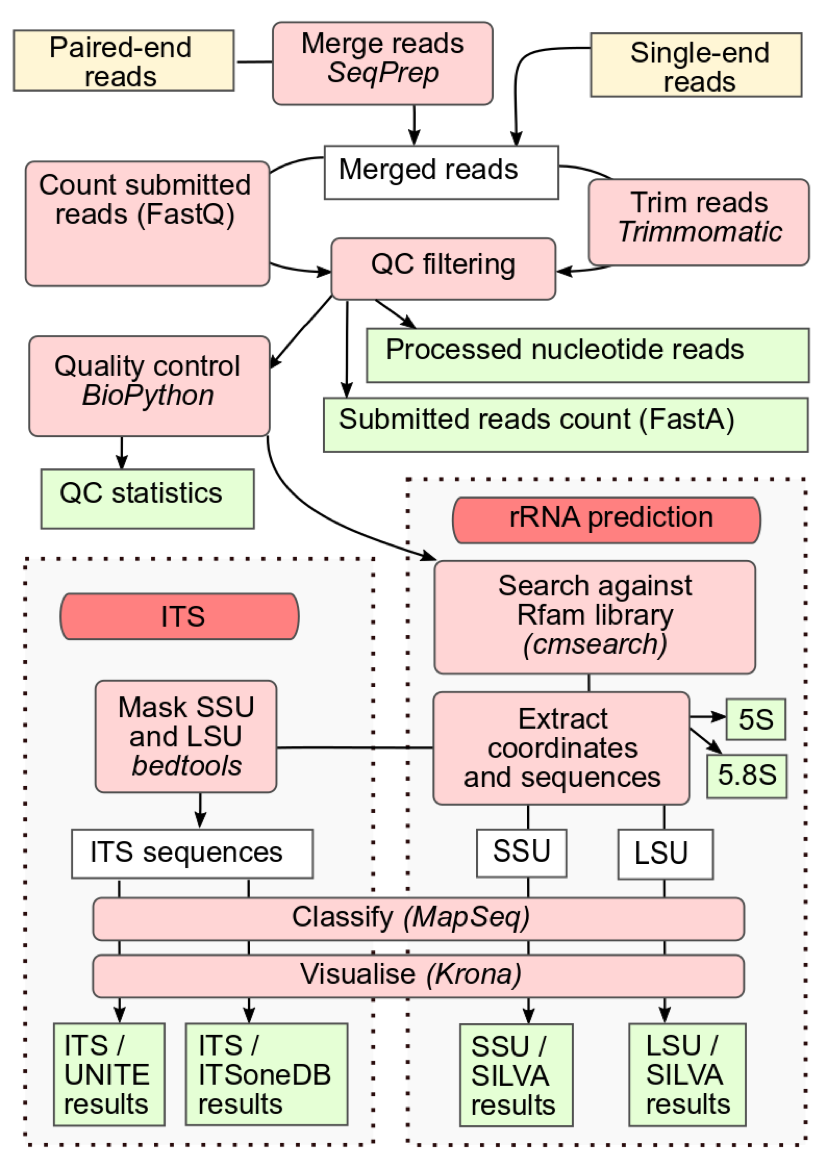
\includegraphics[scale=0.7]{figures/mgnify-workflow-wb.png} }}%
  \captionof{figure}[MGnify's amplicon pipeline]{\textbf{MGnify's amplicon pipeline v5.0}. The flowchart illustrates the workflow of MGnify's amplicon pipeline, with the rRNA-prediction subworkflow enclosed within a dotted box on the right~\cite{noauthor_mgnify_nodate-25}.} \label{fig:amplicon-pipline}%
\end{figure}
\subsection{CMsearch}\label{sec:CMsearch}

\subsubsection{CMsearch}\label{subsubsec:CMsearch}
CMsearch is a command-line tool from the infernal package. Which receives a sequence database and a covariance model (CM) file as inputs. Covariance models are probabilistic models designed to incorporate both the primary sequence and secondary structure of RNA sequences within a family. CMsearch conducts a search against the database, and generates a list of top scoring hits and hit alignments, ranked by E-values~\cite{nawrocki_infernal_2013}. E-values are computed for every alignment hit, providing an estimate of statistical significance for each match~\cite{kalvari_non-coding_2018}.
\subsubsection{CMsearch-deoverlap}\label{subsubsec:CMsearch-deoverlap}
In the MGnify Amplicon pipeline v5.0, the step after CMsearch involves utilizing CMsearch-deoverlap v0.08. It is a perl script (by Eric Nawrocki), that removes low score overlapping hits from the CMsearch output, which are found in the same clan~\cite{nawrocki_nawrockiecmsearch_tblout_deoverlap_2023}.
\subsection{MAPseq}\label{subsec:MAPseq}
MAPseq is a quick and accurate tool that assigns taxonomy and Operational taxonomic unit (OTU) classifications to rRNA sequences~\cite{rodrigues_mapseq_2023}. It provides multiple taxonomy classifications and OTU mappings in a single run. MAPseq is 10 times faster than NINJA-OPS and 100 times faster than VSEARCH with 30\%\ higher accuracy in genus classification compared to other tools. MAPseq outperforming the other tools in most of the tests is attributed to improvements in k-mer counting, including an initial pre-clustering step, Needleman-Wunsch alignment for high-scoring segment pairs, and the computation of classification confidence~\cite{matias_rodrigues_mapseq_2017}. The source code and binary packages are freely accessible on GitHub~\cite{rodrigues_mapseq_2023}.


\section{Kraken v2}\label{sec:Kraken}
Kraken v2 is a k-mer-based taxonomic classification tool. It is the improved version of Kraken v1, it consumes 85\%\ less memory, is five times faster than Kraken v1, and still maintains high accuracy~\cite{wood_improved_2019}. These improvements are achieved by replacing the previously employed sorted list of k-mer/LCA (Lowest Common Ancestor) pairs, which was indexed by minimizers, with a more efficient probabilistic and compact hash table that maps minimizers to their respective LCAs~\cite{wood_improved_2019}. In contrast to Kraken v1, storing all k-mers, the data structure of Kraken v2 stores only the minimizers corresponding to every k-mer~\cite{wood_improved_2019}.
\\
The default taxonomy database used in combination with Kraken v2 is the NCBI database, it also supports three non-NCBI taxonomy based databases, such as Greengenes 16S sequences database, RDP 16S database, and SILVA SSU Ref NR 99. Additionally, a custom database can be build using known taxonomies~\cite{noauthor_kraken2docsmanualmarkdown_nodate}.
\\
In a study conducted by Lu and Salzberg in 2020, a comparison was made among Kraken v2, Bracken v2.5, and QIIME 2 v2017.11, all used in conjunction with the RDP 11.5, SILVA 132, and Greengenes v13\textunderscore8 databases. These tools were evaluated using the same simulated data-sets from a study by Almeida \emph{et al.}~\cite{almeida_benchmarking_2018}. The findings of the study revealed that Kraken v2 and Bracken significantly outperformed QIIME~2 in terms of database build time for the Greengenes and SILVA databases, being up to 100 times faster. Furthermore, in terms of classification time, Kraken v2 and Bracken were up to 300 times faster, consumed up to 100 times less RAM, and demonstrated higher 16S rRNA profiling accuracy compared to QIIME~2~\cite{lu_ultrafast_2020}.\\
Another recent study by Odom \emph{et al.} compared Kraken v2, Mothur, PathoScope~2, QIIME~2, and DADA~2, in conjunction with Greengenes v13\textunderscore8, Kraken v2, SILVA v138, and Refseq v2020 reference databases. The study was conducted using 16S simulated samples retrieved from multiple sources. The study's results showed that the whole-genome metagenomics tools Kraken v2 and PathoScope~2, demonstrated better performance than the 16S analyses tools DADA~2, QIIME~2, and Mothur~\cite{odom_metagenomic_2023}.
\section{SILVA-database}\label{sec:SILVA}
SILVA is an ever-expanding online collection of databases containing quality-checked rRNA sequences~\cite{quast_silva_2013}. In February 2007, its initial release 89 contained 353,366 SSU sequences and 46,979 LSU sequences~\cite{noauthor_release_nodate-1}. The last release v138.1 (August 2020) comprises 9,469,124 SSU sequences and 1,312,534 LSU sequences~\cite{noauthor_release_nodate}. The database is periodically issued as releases, rather than undergoing continuous updates, with the aim of enabling comparability of studies making use of the SILVA database. The data is derived from the EMBL-Bank, each SILVA release is assigned a number corresponding to the EMBL-Bank release from which it originates~\cite{quast_silva_2013}. 
\\
The SILVA databases serve as the official databases for ARB, a software package  employed for database handling and data analysis. The databases are available for download via the SILVA website in either ARB or FASTA format files. This flexibility allows researchers to integrate SILVA with the usage of various pipelines/tools such as QIIME, Mothur etc.~\cite{quast_silva_2013}.
\\
SILVA offers three distinct database categories for both SSU and LSU sequences. Firstly, the Parc database encompasses all sequences available in SILVA. Second, the Ref database, which is a refined subset of the Parc database, containing only high-quality sequences. Lastly, the Ref NR 99 database, derived from the Ref database by excluding sequences that share 99\%\ or more similarity with one another~\cite{noauthor_release_nodate}.
\\
A Benchmark conducted by Almeida \emph{et al}. compared taxonomic classifiers (MAPseq v1.2.2, mothur v1.39.5, QIIME v1.9.1, and QIIME 2 v2017.11) in conjunction with diverse databases (Greengenes v13\textunderscore8, SILVA v128, RDP v16, and NCBI mapref v2.2) using simulated samples. The findings of this research revealed that SILVA generally demonstrated superior recall rates at the family and genus ranks. Moreover, SILVA had better accuracy in predicting the true composition of the mock samples~\cite{almeida_benchmarking_2018}.
\section{Krona}\label{sec:Krona}
Krona is a visualization tool designed to craft pie charts for visualizing hierarchical data such as taxonomic abundance. Leveraging HTML5 and JavaScript, Krona's charts offer interactivity (\Cref{fig:krona_example}), can be displayed in a web browser, and facilitate effortless sharing among users~\cite{ondov_interactive_2011}.
\chapter{Methods}\label{chap:Methods}

\section{MGnify's rRNA-prediction subworkflow}\label{sec:Ported-version-of-MGnify}

\subsection{Detailed step-by-step analysis of the MGnify rRNA-prediction subworkflow}\label{subsec:Interpretation}
To facilitate the interpretation of the rRNA-prediction subworkflow, the CWL scripts~\cite{noauthor_pipeline-v5_2023} and CWL-Viewer tool~\cite{noauthor_common_nodate} were employed to investigate the subworkflow. Furthermore, the subworkflow was visualized (\Cref{fig:rRNA-prediction-subWF}) using the online visualization application drawio~\cite{noauthor_jgraphdrawio_nodate}.\\
A detailed step-by-step description of the subworkflow is shown in \Cref{fig:rRNA-prediction-subWF}. The workflow comprises the following steps: CMsearch conducts a similarity search using the quality-checked reads (input\textunderscore sequences) and Rfam SSU and LSU covariance models, and outputs a ranked list of top-scoring hits and hit alignments (matches). The matches of CMsearch and a clan information file, a file containing a list of clans, CL00111 (SSU) and CL00112 (LSU), are directed to cmsearch-deoverlap. Cmsearch-deoverlap removes low-score overlapping hits from the CMsearch output, which are found in the same clan and outputs deoverlapped matches. The awk based script extract\textunderscore coords\textunderscore awk extracts the target sequence name, accession number, sequence start, and sequence end from the deoverlapped matches and formats them to be suitable as an input for esl-sfetch-manyseqs. Esl-sfetch-manyseqs, a tool used to extract sequences or subsequences from an indexed sequences file~\cite{eddy_hmmer_nodate},  receives the sequences matched with their coordinates as well as the indexed sequence file in SSI format from esl-sfetch-index and outputs a FASTA file containing the sliced sequences. Get\textunderscore subunits extracts the SSU and LSU sequences and separates them into two different FASTA files. MAPseq classifies the SSU and LSU sequences, using the corresponding SILVA SSU/LSU database and SSU/LSU taxonomy file. Mapseq2biom receives the classifications from MAPseq and the corresponding SILVA SSU/LSU OTU table, and 
produces three outputs: A TSV file (otu\textunderscore tsv) containing OTU IDs, abundance, taxonomy, and NCBI taxonomy IDs. A second TSV file (otu\textunderscore tsv\textunderscore notaxid) excluding the NCBI taxonomy IDs. And a third file (otu\textunderscore txt) containing abundance and taxonomy, that serves as a Krona input. Biom convert is used to convert otu\textunderscore tsv\textunderscore notaxid to HDF5 and JSON formats. Lastly, Krona visualizes the taxa abundance table  (otu\textunderscore txt) in the form of a relative abundance pie chart.

\begin{figure}[H]
  \centering
  \subfloat{{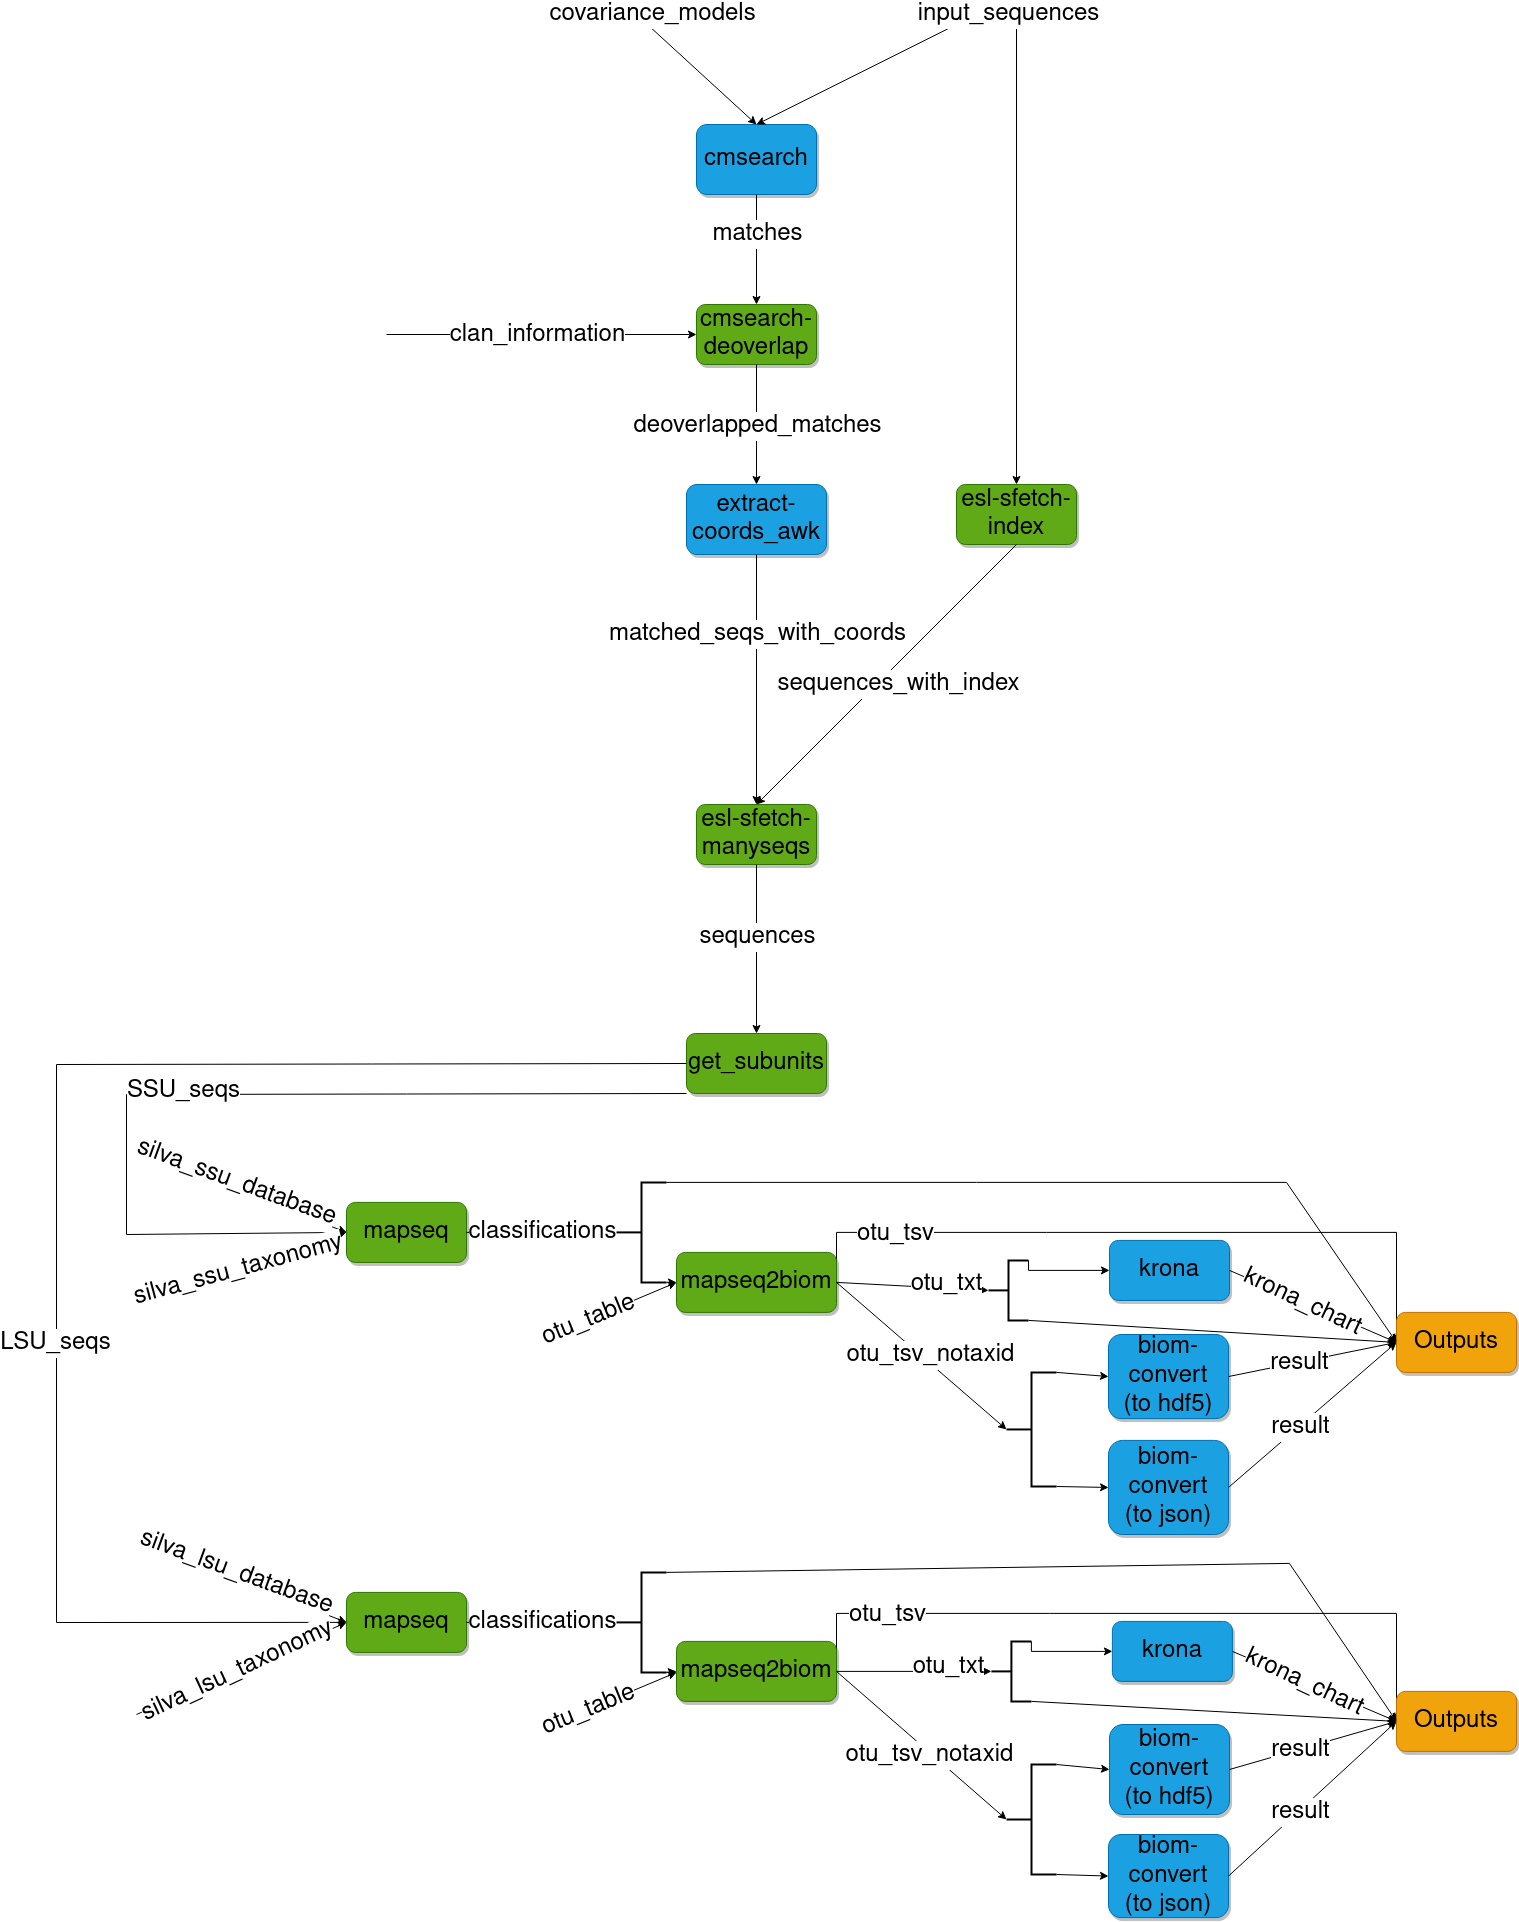
\includegraphics[scale=0.26]{figures/flowchart_rnaPredictionSubWF.drawio.png} }}%
  \captionof{figure}[MGnify's rRNA-prediction subworkflow]{\textbf{MGnify's rRNA-prediction subworkflow}. Visualized using drawio. The blue boxes show tools already existing in Galaxy. The green boxes show the tools, which were missing from Galaxy.} \label{fig:rRNA-prediction-subWF}%
\end{figure}

\subsection{Port of the rRNA-prediction subworkflow into Galaxy}\label{subsec:Ingration_to_galaxy}
Tools that were not available in Galaxy were identified. The identified tools were either replaced by existing Galaxy tools with similar functions, or a Galaxy wrapper was developed for the missing tools. Planemo, a set of command-line utilities designed to support Galaxy tool development~\cite{noauthor_welcome_nodate}, was used to test and lint the developed tool wrappers.\\
The existing wrappers for CMsearch (from the infernal package v1.1.4) had minor mistakes, which resulted in undesired Outputs~\cite{gruning_galaxy_2023}; small adjustments had to be conducted before use. CMsearch-deoverlap v0.08~\cite{nawrocki_nawrockiecmsearch_tblout_deoverlap_2023} was wrapped and integrated into Galaxy~\cite{noauthor_galaxytoolstoolsrna_toolscmsearch_deoverlap_nodate}.\\
Esl-sfetch was substituted with the functionally similar tool bedtools getfasta~\cite{noauthor_tools-iuctoolsbedtools_nodate}, which already existed as galaxy tool. In order to be able to use bedtools getfasta instead of esl-sfetch, the output created by cmsearch-deoverlap (see \Cref{fig:rRNA-prediction-subWF}) had to be formatted and converted to a regions file in BED format. The conversion was made using the Galaxy tools: Query Tabular~\cite{noauthor_tools-iuctoolsquery_tabular_nodate}, Text reformatting~\cite{noauthor_galaxytoolstoolstext_processingtext_processing_nodate}, and Concatenate two BED files~\cite{noauthor_tools-devteamtool_collectionsgopsconcat_nodate}.\\
Since the version of MAPseq~\cite{rodrigues_mapseq_2023} used by MGnify (v1.2.3), was not available on bioconda, the latest version 2.1.1 ~\cite{noauthor_mapseq_nodate} was adopted for the wrapper~\cite{noauthor_tools-iuctoolsmapseq_nodate}. Furthermore, the tool mapseq2biom~\cite{noauthor_pipeline-v5toolsrna_predictionmapseq2biommapseq2biompl_nodate} was included as an option in the MAPseq wrapper (\Cref{fig:MAPseq}).\\
The Galaxy wrapper for Krona v2.7.1~\cite{noauthor_tools-iuctoolstaxonomy_krona_chart_nodate} existed already and was adopted as-is (\Cref{fig:rRNA-prediction-subWF,fig:Galaxy_WF_part2}).\\
 Biom convert (from the biom-format package v2.1.14~\cite{noauthor_tools-iuctoolsbiom_format_nodate}) had minor mistakes, which resulted in Errors or undesired Outputs~\cite{noauthor_galaxy_2023}; small adjustments had to be conducted before use (\Cref{fig:rRNA-prediction-subWF,fig:Galaxy_WF_part2}).\\



\section{Benchmark}\label{sec:Benchmark}


\subsection{Benchmark Set-Up}\label{subsec:Benchmark-Set-Up}

\subsubsection{MGnify samples benchmark Workflow}\label{subsubsec:Benchmark-Workflow-mgnify}
The FASTA files containing the SSU quality checked reads and the analysis result files were downloaded from MGnify's website. The focus was exclusively on SSU reads to align with the scope of the bachelor thesis. As the published results on MGnify's website did not contain a Krona-compatible input file, one was formatted for each sample from the OTU table (otu\textunderscore tsv).
The FASTA files and publicly available MGnify-compatible database files~\cite{noauthor_index_nodate} were subsequently uploaded to Galaxy. Where the FASTA files were packed into a data-set collection, and served as the input for the RNA-prediction subworkflow on Galaxy.\\
After executing the subworkflow on Galaxy, the Krona inputs from both Galaxy and MGnify were grouped by taxonomy rank, and their abundances were aggregated. Subsequently, the tables were joined based on the taxon column. These combined tables featured a first column for taxon names, a second column for the corresponding MGnify abundances for each taxon, and a third column for the corresponding Galaxy abundances. These tables were employed as the input for calculating the beta diversity metrics, specifically the Bray-Curtis and Jaccard distances. The beta diversity workflow can be found in \Cref{appendix_galaxy_workflows}. This data was subsequently visualized in the form of plots (\Cref{fig:mgnify_human_gut_beta_div,fig:mgnify_soil_beta_div}). Scripts used for plotting the data can be found in \Cref{appendix_results}.\\
Additionally, relative abundance tables, using total-sum scaling (TSS), were generated for the species and genus ranks taxonomic data in both soil and human large intestine samples. The computed relative abundance tables of MGnify and Galaxy were subsequently merged. Taxa in the output of Galaxy port different to MGnify were excluded to highlight the discrepancy in the resulting plots~(\Cref{fig:mgnify_human_gut_rel_abundance_s_level,fig:mgnify_soil_rel_abundace_s_level}).\\
Furthermore, summary tables were generated including abundance, taxa as row indexes, and analysis IDs as column indexes.\par
MGnify's quality-checked reads were additionally classified using Kraken v2, using its default configuration. Since SILVA 16S v132 for use with Kraken v2 was absent in Galaxy, Kraken v2 was used in conjunction with SILVA 16S v138. Kraken v2 report files were generated for subsequent conversion into Krona-compatible input files using the kreport2krona tool from the krakentools package~\cite{noauthor_tools-iuctoolskrakentools_nodate}. However, it is worth noting that Kraken v2's taxonomic lineage consists only of starting from kingdom and to genus ranks. Adjustments were made to align MGnify's output with this specific taxonomic lineage. 
Subsequently, the beta diversity values were calculated and visualized in a similar manner as forementioned.

\subsubsection{Mock samples benchmark Workflow}\label{subsubsec:Benchmark-Workflow-mock}

Mock samples mentioned in \Cref{subsubsec:mock_samples} and their corresponding BIOM results files were downloaded. The FASTQ files were converted to FASTA format and subjected to classification twice: once using the rRNA-prediction subworkflow on Galaxy and the other using Kraken v2.
The BIOM files contained taxonomic data, sample-analysis-IDs, expected abundance for each taxon, and the corresponding abundance values from different runs with each tool, all in conjunction with various databases. The samples and their expected taxonomic composition were extracted from the BIOM files and formatted to match Krona input file format. Given the taxonomic lineage of the mock samples and Kraken v2 consist only of ranks starting from kingdom and concluding with genus, outputs of Galaxy's rRNA-prediction subworkflow were adjusted to match this lineage.
Subsequently, procedures similar to those mentioned in \Cref{subsubsec:Benchmark-Workflow-mgnify}, were employed to generate beta diversity and relative abundance plots. Taxa in the outputs of Galaxy-port and Kraken v2 different to the expected taxonomic composition were excluded to highlight the discrepancy in the resulting plots.

\subsubsection{Dissimilarity Measures}\label{subsubsec:Dissimilarity-Measures}

Beta diversity is a measure that quantifies the dissimilarity between microbial environments based on taxonomic composition. This thesis employed the Bray-Curtis and Jaccard distance beta diversity metrics, to assess the differences between the results of the different pipelines/tools. Beta diversity was also employed to assess the differences between the achieved results of the Galaxy ported version and Kraken v2 using the mock samples. The beta diversity measurements using the different metrics were applied on the whole abundance table of each output, and also on each taxonomic rank separately.\\
Bray Curtis is a quantitative beta diversity metric, based on occurrence data (abundance). The Bray Curtis distance quantifies the dissimilarity between two samples, A and B by employing the equation:
\[
BC(A,B) = \frac{\sum_{i}^{} |X_{iA} - X_{iB}|}{\sum_{i}^{} X_{iA} + X_{iB}} \tag*{\cite{ricotta_properties_2017}}
\]

Where:
\begin{itemize}
    \item \(X_{iA}\) represents the frequency of taxon \(i\) in sample A.
    \item \(X_{iB}\) represents the frequency of taxon \(i\) in sample B.
\end{itemize}
Jaccard distance is a qualitative beta diversity metric measuring the dissimilarity between samples, with focus on the presence/absence of taxa, regardless of their abundance.\\ Given two taxa sets A and B, Jaccard distance is calculated by employing the equation:
\[
J(A,B) = 1 - \frac{|A \cap B|}{|A \cup B|} \tag*{\cite{levandowsky_distance_1971}}
\]
\subsection{Sample selection}\label{subsec:Sample-Selection}
\subsubsection{MGnify samples}\label{subsubsec:mgnify_samples}
For the benchmark of MGnify's rRNA-prediction subworkflow against its Galaxy-ported version and Kraken v2, a selection of 10 human large intestine samples (\Cref{tab:human-gut-samples}), and 10 soil samples (\Cref{tab:soil-samples}) were randomly gathered from MGnify. All gathered samples are from previous MGnify amplicon analyses and contain only SSU sequences. Processed nucleotide reads (after quality control) were acquired for each sample and analyzed using both the ported MGnify version and Kraken v2.
\\
\begin{table}[H]
    \centering
    \begin{tabular}{|c |c| c |c|} 
 \hline
 Analysis & Sample & MGnify ID & Ref. \\ [0.5ex] 
 \hline\hline
 MGYA00564861 & ERS4804749 & MGYS00005591 & ~\cite{noauthor_mgnify_nodate-19} \\ 
 \hline
 MGYA00564896 & ERS4804701 & MGYS00005591 & ~\cite{noauthor_mgnify_nodate-18} \\
 \hline
 MGYA00566149 & ERS3014381 & MGYS00005601 & ~\cite{noauthor_mgnify_nodate-17} \\
 \hline
 MGYA00566193 & ERS3014355 & MGYS00005601 & ~\cite{noauthor_mgnify_nodate-16} \\
 \hline
 MGYA00574359 & ERS581082 & MGYS00005628 & ~\cite{noauthor_mgnify_nodate-15} \\ 
 \hline
 MGYA00574498 & ERS581039 & MGYS00005628 & ~\cite{noauthor_mgnify_nodate-14} \\
 \hline
 MGYA00583678 & DRS070813 & MGYS00005742 & ~\cite{noauthor_mgnify_nodate-13} \\
 \hline
 MGYA00584014 & DRS070789 & MGYS00005742 & ~\cite{noauthor_mgnify_nodate-12} \\
 \hline
 MGYA00585042 & SRS4172095 & MGYS00005755 & ~\cite{noauthor_mgnify_nodate-11} \\
 \hline
 MGYA00585118 & SRS4172137 & MGYS00005755 & ~\cite{noauthor_mgnify_nodate-10} \\ [1ex]
 \hline
\end{tabular}
    \caption[MGnify Human large intestine samples]{\textbf{MGnify Human large intestine samples}. Ten human large intestine quality-checked FASTA and their corresponding results retrieved from MGnify's website. Exclusively from SSU analysis.}
    \label{tab:human-gut-samples}
\end{table}



\begin{table}[H]
    \centering
    \begin{tabular}{|c |c| c |c|} 
 \hline
 Analysis & Sample & MGnify ID & Ref. \\ [0.5ex] 
 \hline\hline
 MGYA00553054 & SRS825517 & MGYS00005241 & ~\cite{noauthor_mgnify_nodate-9} \\ 
 \hline
 MGYA00573072 & ERS1798652 & MGYS00001864 & ~\cite{noauthor_mgnify_nodate-8} \\
 \hline
 MGYA00578739 & SRS825501 & MGYS00005241 & ~\cite{noauthor_mgnify_nodate-7} \\
 \hline
 MGYA00578910 & SRS825629 & MGYS00005241 & ~\cite{noauthor_mgnify_nodate-6} \\
 \hline
 MGYA00573077 & ERS1798633 & MGYS00001864 & ~\cite{noauthor_mgnify_nodate-5} \\ 
 \hline
 MGYA00565430 & SRS726304 & MGYS00001031 & ~\cite{noauthor_mgnify_nodate-4} \\
 \hline
 MGYA00523039 & ERS1798534 & MGYS00001864 & ~\cite{noauthor_mgnify_nodate-3} \\
 \hline
 MGYA00578954 & SRS825558 & MGYS00005241 & ~\cite{noauthor_mgnify_nodate-2} \\
 \hline
 MGYA00523976 & ERS1799257 & MGYS00001864 & ~\cite{noauthor_mgnify_nodate-1} \\
 \hline
 MGYA00523193 & ERS1798753 & MGYS00001864 & ~\cite{noauthor_mgnify_nodate} \\ [1ex]
 \hline
\end{tabular}
    \caption[MGnify soil samples]{\textbf{MGnify soil samples}. Ten soil quality-checked FASTA files and their corresponding results retrieved from MGnify's website. Exclusively from SSU analysis.}
    \label{tab:soil-samples}
\end{table}

\par
\subsubsection{Mock samples}\label{subsubsec:mock_samples}
Several 16S SSU mock samples, from Almeida \emph{et al.}~\cite{almeida_benchmarking_2018}, were also used to serve as a benchmark for comparing the Galaxy-ported version of MGnify with Kraken v2. The samples are publicly available~\cite{noauthor_index_nodate}. A mock sample is a synthetically generated sample, wherein the composition of various taxa is predetermined. Having an expected taxonomic composition offers an advantage during the benchmarking process, facilitating the identification of dissimilarities. The used samples were: A100\textunderscore V34\textunderscore 10K\textunderscore 1\textunderscore human-gut, A100\textunderscore V34\textunderscore 10K\textunderscore 1\textunderscore soil, A100\textunderscore V4\textunderscore 10K\textunderscore 1\textunderscore human-gut, A100\textunderscore V4\textunderscore 10K\textunderscore 1\textunderscore soil. These samples contain 100 random species belonging to the 80 most abundant genera in these communities. The decision was made to incorporate only samples with V3-V4 and V4 primers, since these achieved the highest percentage of sequence retrieval~\cite{almeida_benchmarking_2018}, also to assure a comparison fairness with Kraken v2, which uses only 16S of SILVA v138.
\chapter{Results}\label{chap:Results}
\section{Ported rRNA-prediction subworkflow}\label{results_subworkflow integration}
The ported rRNA-prediction subworkflow is shown in \Cref{fig:Galaxy_WF_part1,fig:Galaxy_WF_part2}.\\
The tool cmsearch-deoverlap v0.08 was successfully XML-wrapped and integrated into Galaxy.\\
The deoverlapped CMsearch matches are formatted into BED files. Query Tabular is used to extract the target SSU sequence name, start location, and end location. When the direction is 'forward,' the columns are selected in their existing order, while in the 'reverse' direction, the start and end location columns are swapped. The awk based text formatting tool is utilized to adjust the start location indexing and append the direction to each line. Subsequently the 'forward' and 'reverse' BED files are concatenated into a single BED file. The analogues procedure is also employed for LSU sequences. The resulting SSU and LSU BED files are directed to bedtools getfasta, which extracts the sequences from the quality-checked reads file.\\
The integration of MAPseq v2.1.1 and mapseq2biom was successful. These two tools were merged into one tool wrapper. \Cref{fig:MAPseq} illustrates the interface of MAPseq within Galaxy. Users have the option to select between cached database files or upload their own database files. The cached databases include the SSU and LSU SILVA v132 MGnify-compatible database files, which are made accessible through a data manager. Mapseq2biom was added as an option (Outlined in red in \Cref{fig:MAPseq}).\\
The remainder of the rRNA-prediction subworkflow (\Cref{fig:Galaxy_WF_part1,fig:Galaxy_WF_part2}) was constructed in the same manner as detailed in \Cref{subsec:Interpretation}.


\begin{landscape}

\begin{center}
  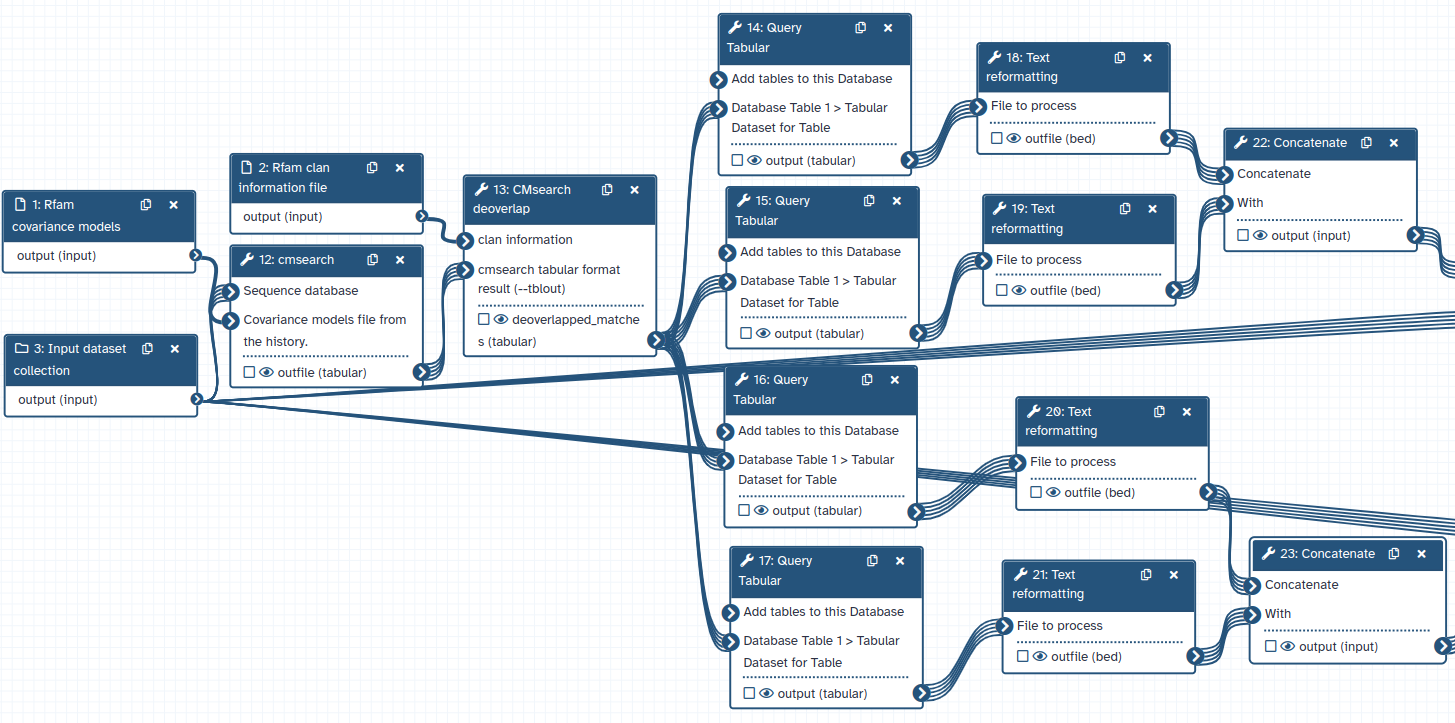
\includegraphics[width=\paperwidth,height=\paperheight,keepaspectratio]{figures/Galaxy_WF_part1.png}
  \captionof{figure}[Galaxy-ported version of rRNA-prediction subworkflow (part 1)]{\textbf{Galaxy-ported version of rRNA-prediction subworkflow (Part 1)}. The initial part of the rRNA-prediction subworkflow within the Galaxy interface. The link to the Galaxy-ported rRNA-prediction subworkflow can be found in \Cref{appendix_galaxy_workflows}} \label{fig:Galaxy_WF_part1}%
\end{center}

\end{landscape}
\begin{figure}[H]
  \centering
  \subfloat{{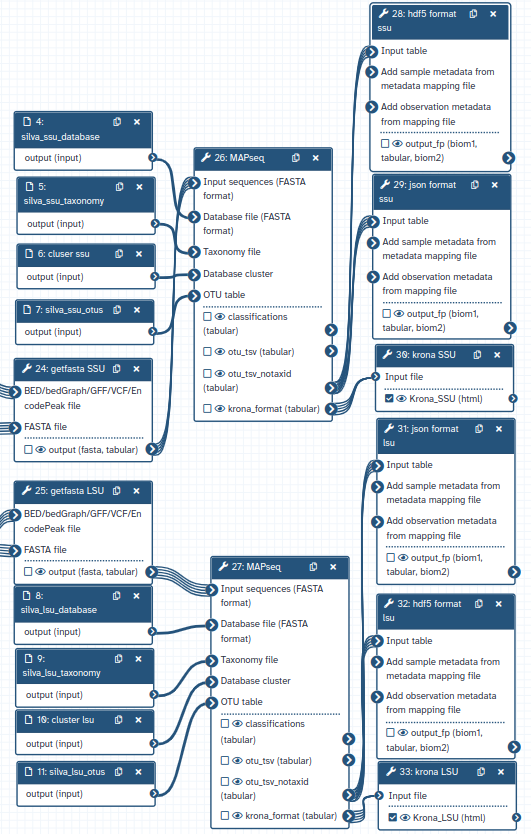
\includegraphics[scale=0.6]{figures/Galaxy_WF_part2.png} }}%
  \captionof{figure}[Galaxy-ported version of rRNA-prediction subworkflow (part 2)]{\textbf{Galaxy-ported version of rRNA-prediction subworkflow (Part 2)}. The second part of the rRNA-prediction subworkflow within the Galaxy interface. Where getfasta SSU and getfasta LSU receive the SSU and LSU BED files from Concatenate (Tool IDs 22 and 23 in \Cref{fig:Galaxy_WF_part1})} \label{fig:Galaxy_WF_part2}%
\end{figure}
\begin{figure}[H]
  \centering
  \subfloat{{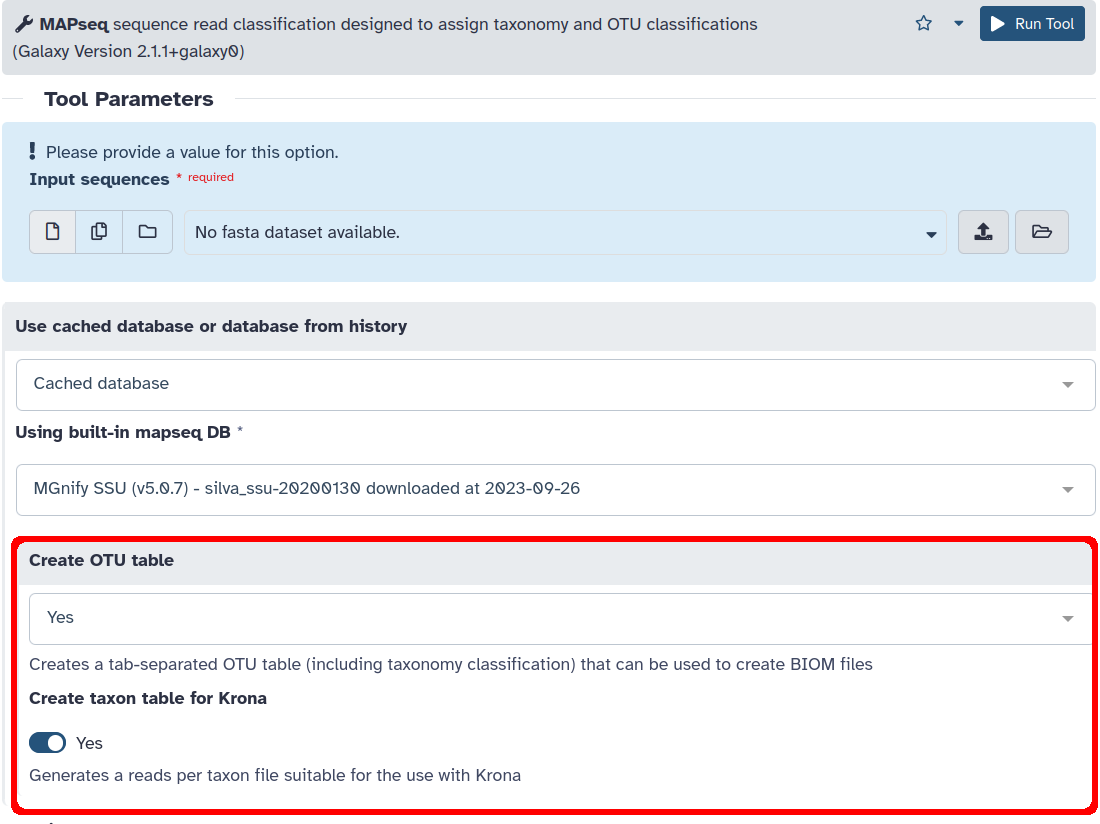
\includegraphics[scale=0.36]{figures/MAPseq.png} }}%
  \captionof{figure}[MAPseq tool in Galaxy]{\textbf{GUI view of the MAPseq tool in Galaxy}~\cite{noauthor_tools-iuctoolsmapseq_nodate}. including the mapseq2biom tool as an option (outlined in red).} \label{fig:MAPseq}%
\end{figure}
\section{MGnify samples benchmark}\label{sec:MGnify's samples}
\subsection{Benchmark of Galaxy-ported rRNA-prediction subworkflow pipeline against its MGnify counterpart}\label{subsec:mgnifyVSgalaxy}
The results for the benchmark of samples from two different biomes, human large intestine and soil, are shown in \Cref{fig:mgnify_human_gut_beta_div,fig:mgnify_soil_beta_div}. These figures provide a graphical presentation of dissimilarity values computed using the two metrics, Bray Curtis distance and Jaccard distance, at each taxonomic rank, as well as for all ranks combined.
Two trends can be observed in the beta diversity plots (\Cref{fig:mgnify_human_gut_beta_div,fig:mgnify_soil_beta_div}). First, lower taxonomic ranks show on average, higher dissimilarity values than higher ranks. In both MGnify and Galaxy-port results, the taxonomic ranks of super kingdom and kingdom exhibited identical taxa presence (Jaccard distance equals 0) and nearly identical abundance (Bray Curtis distance of approximately 0). The highest average dissimilarity values were observed at the species rank. The second notable trend involves Jaccard distance values being consistently greater than the Bray Curtis values, from the phylum rank downwards. The second trend was caused by individual taxa having an abundance of 1 in MGnify's results while being absent in Galaxy's results, or vice versa (see example in \Cref{jaccard_example}).
\begin{figure}[H]
  \centering
  \hfill
  \subfloat{{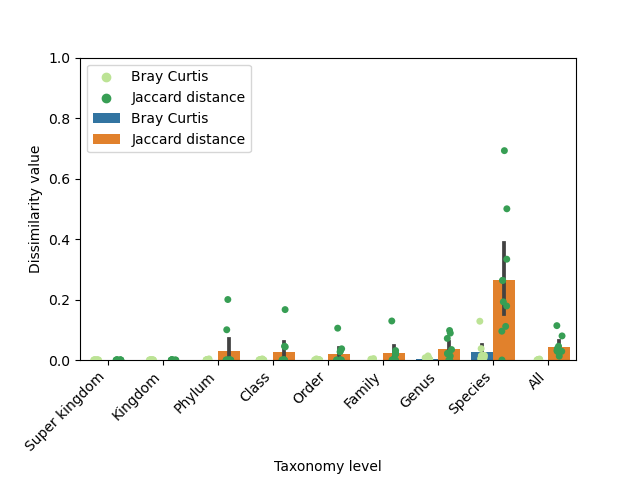
\includegraphics[scale=0.8]{figures/human_gut_plot_galaxyVSmgnify.png} }}%
  \captionof{figure}[Beta diversity-based benchmark. Dissimilarity between MGnify and Galaxy-ported pipeline, for MGnify human large intestine samples]{\textbf{Beta diversity-based benchmark}. Dissimilarity between MGnify and Galaxy-ported pipeline, for MGnify human large intestine samples (\Cref{tab:human-gut-samples}). The term 'All' refers to all ranks combined. Bars represent the average dissimilarity values, while individual data points represent the values for each of the individual samples.} \label{fig:mgnify_human_gut_beta_div}%
\end{figure}

\begin{figure}[H]
  \centering
  \hfill
  \subfloat{{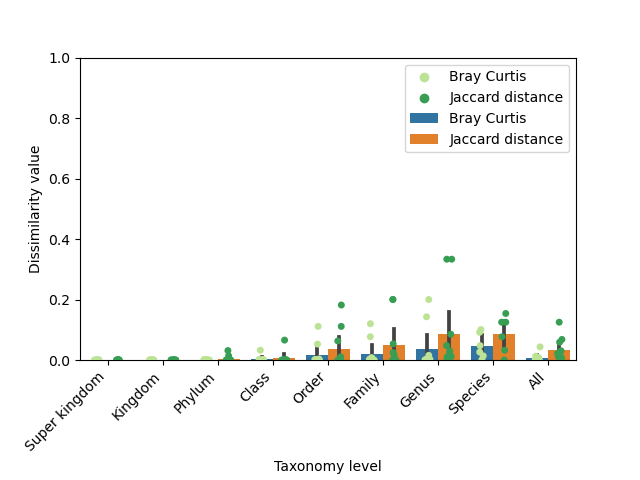
\includegraphics[scale=0.8]{figures/soil_plot_galaxyVSmgnify.png} }}%
  \captionof{figure}[Beta diversity-based benchmark. Dissimilarity between MGnify and Galaxy-ported pipeline, for MGnify soil samples]{\textbf{Beta diversity-based benchmark}. Dissimilarity between MGnify and Galaxy-ported pipeline, for MGnify soil samples (\Cref{tab:soil-samples}). The term 'All' refers to all ranks combined. Bars represent the average dissimilarity values, while individual data points represent the values for each of the individual samples.} \label{fig:mgnify_soil_beta_div}%
\end{figure}
The relative abundance comparison, at genus and species ranks, for MGnify samples for two biomes, human large intestine and soil, is shown in \Cref{fig:mgnify_human_gut_rel_abundance_s_level,fig:mgnify_human_gut_rel_abundance_g_level,fig:mgnify_soil_rel_abundace_s_level,fig:mgnify_soil_rel_abundace_g_level}. Taxa in the output of Galaxy port different to MGnify were excluded to highlight the discrepancy in the resulting plots.
The relative abundance plots (\Cref{fig:mgnify_human_gut_rel_abundance_s_level,fig:mgnify_human_gut_rel_abundance_g_level,fig:mgnify_soil_rel_abundace_s_level,fig:mgnify_soil_rel_abundace_g_level}) show overall good agreement of similarity for taxa with high relative abundance for both of the genus and species ranks. Additionally, in these charts, the Galaxy visual representation showed only isolated small gaps, which indicates only small quantities of taxa were present in Galaxy-port results, yet absent in the MGnify results.\\
The relative abundance plot for soil at the species rank (\Cref{fig:mgnify_soil_rel_abundace_s_level}) concluded only six of the ten benchmarked soil samples. The four absent samples, corresponding to the analyses MGYA00553054, MGYA00578739, MGYA00578910, and MGYA00578954, did not contain any reads at the species rank in either the MGnify or Galaxy-ported results.\\

\begin{figure}[H]
  \centering
  \subfloat{{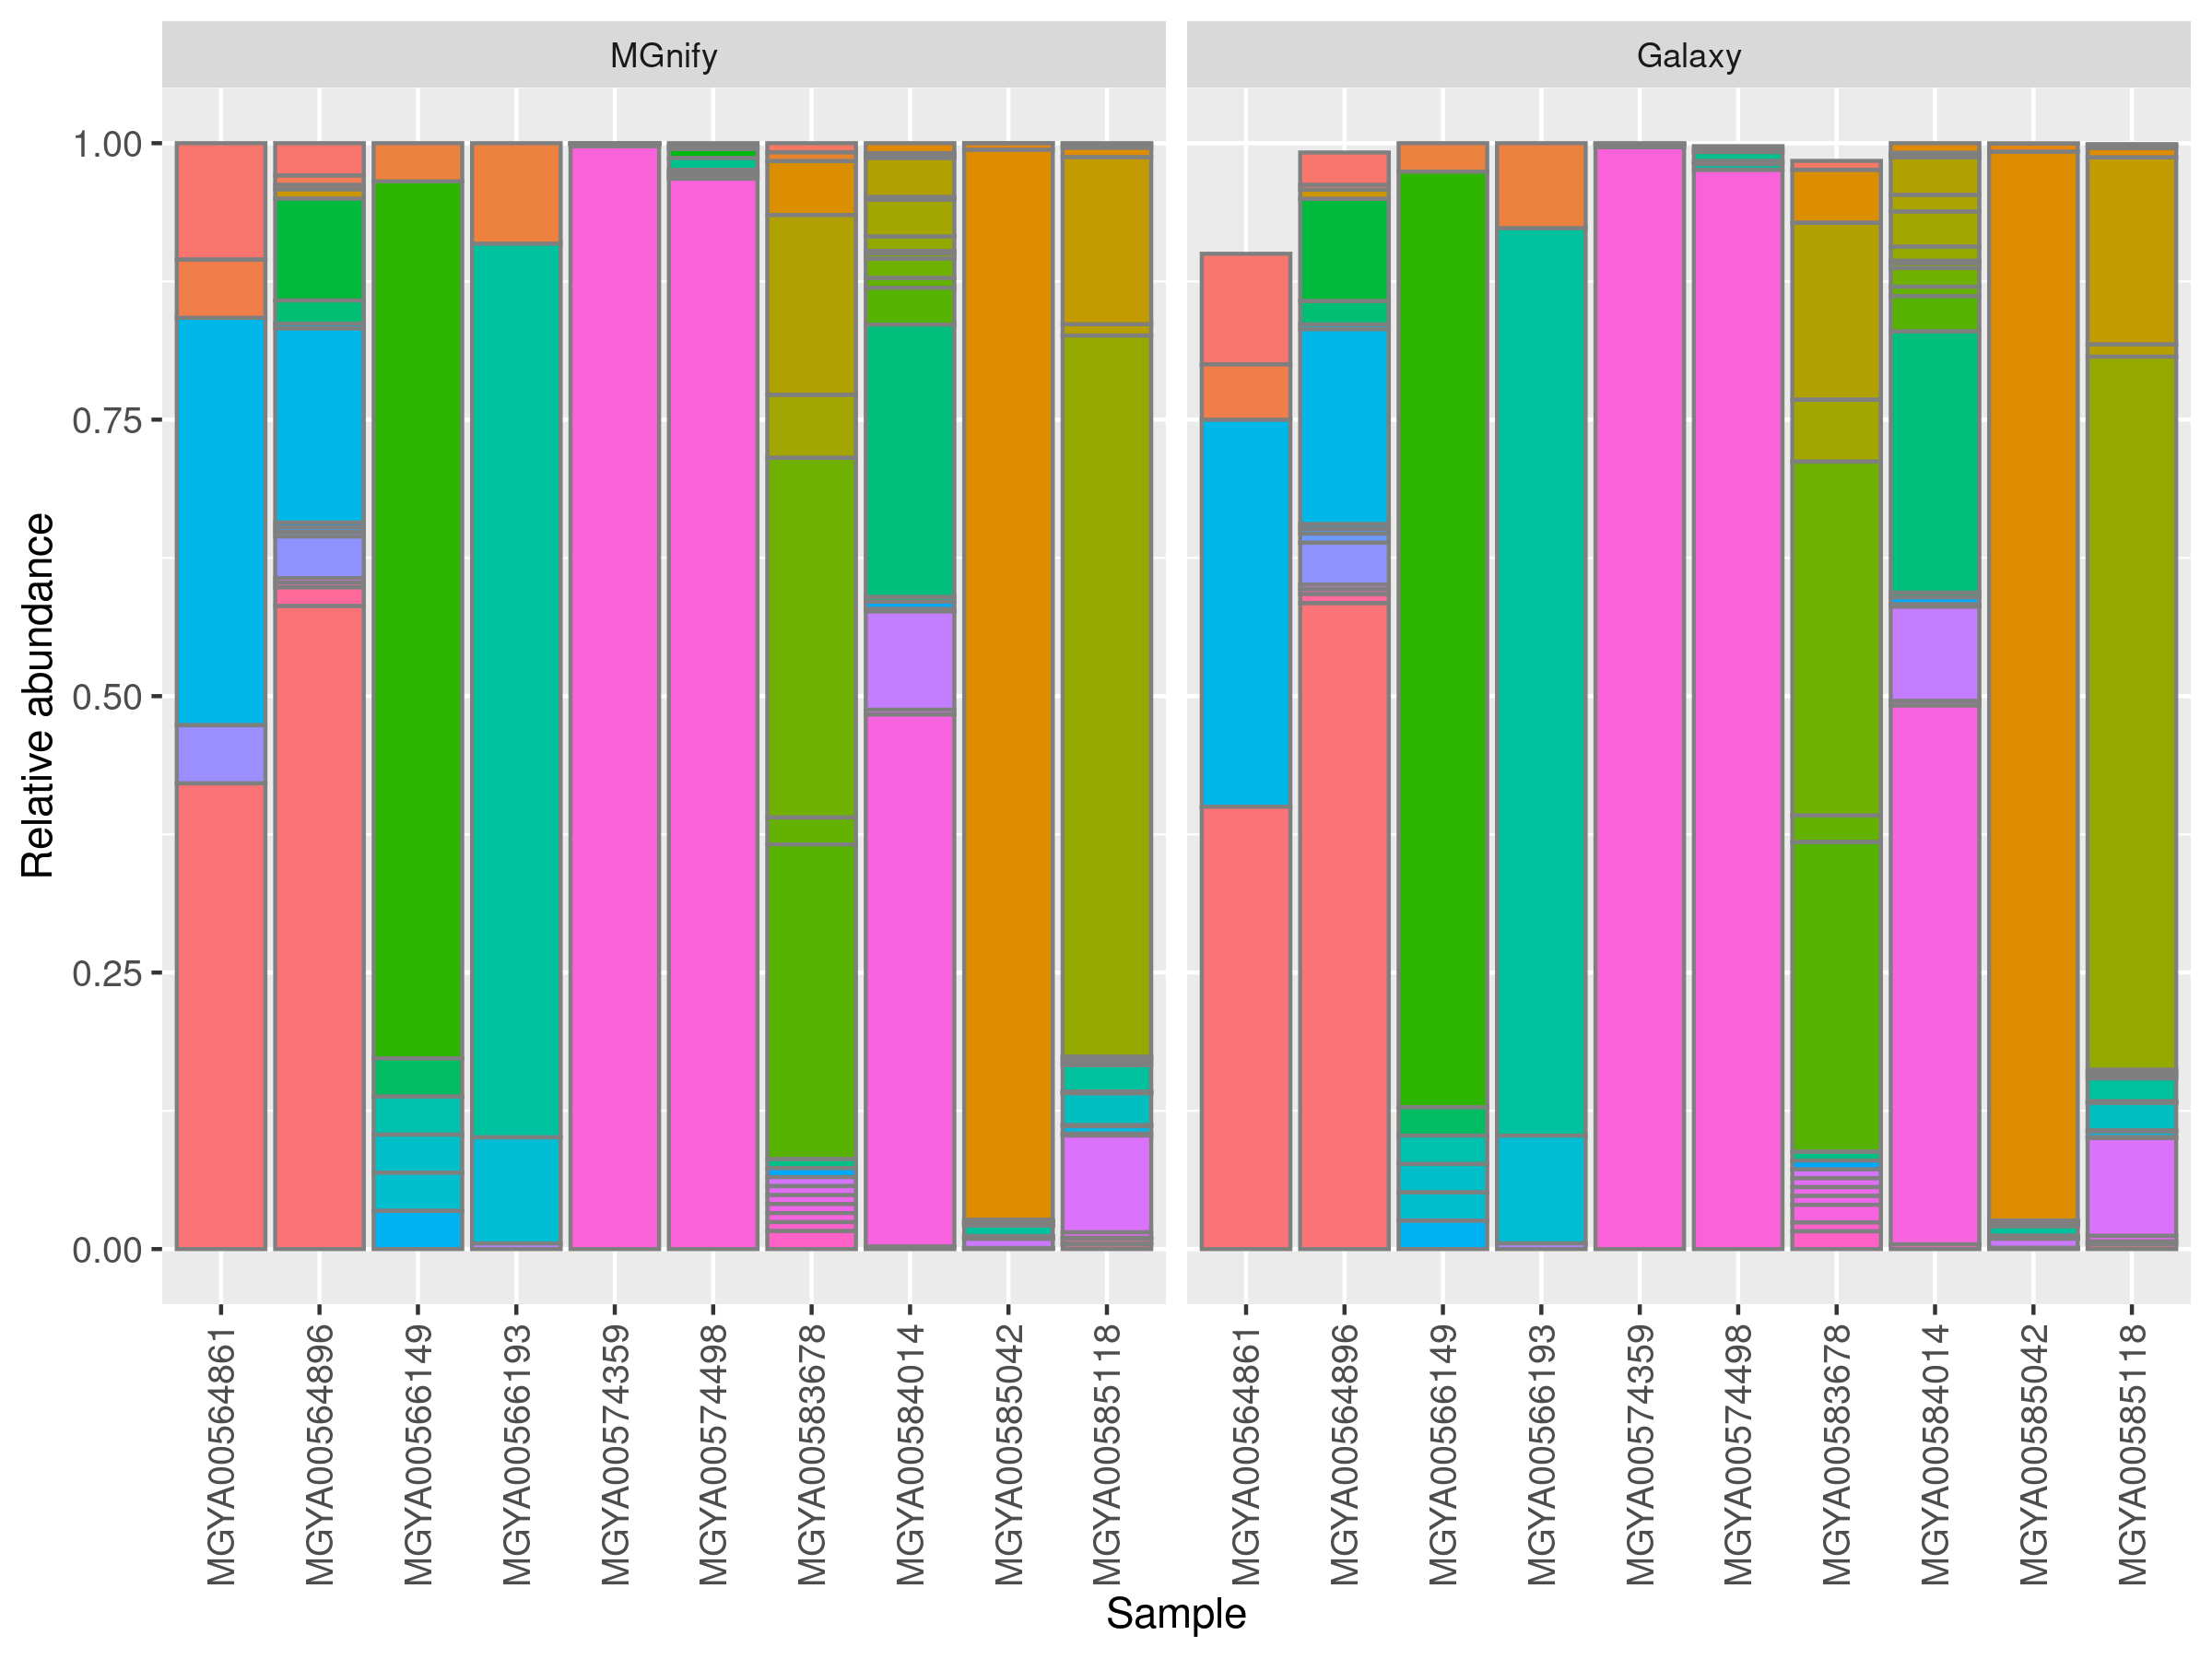
\includegraphics[scale=0.65]{figures/human_gut_abundance_level_s_mgnifyVSgalaxy.png} }}%
  \captionof{figure}[Differences of relative abundance between MGnify and Galaxy-ported pipeline at species rank for MGnify human large intestine samples]{\textbf{Differences of relative abundance between MGnify and Galaxy-ported pipeline at species rank for MGnify human large intestine samples}~(\Cref{tab:human-gut-samples}). Species that were predicted by Galaxy but were not present in the MGnify output are not shown. The plot legend can be found in the appendix (\Cref{fig:human_gut_abundance_level_s_mgnifyVSgalaxy_legend.png})} \label{fig:mgnify_human_gut_rel_abundance_s_level}%
\end{figure}

\begin{figure}[H]
  \centering
  \subfloat{{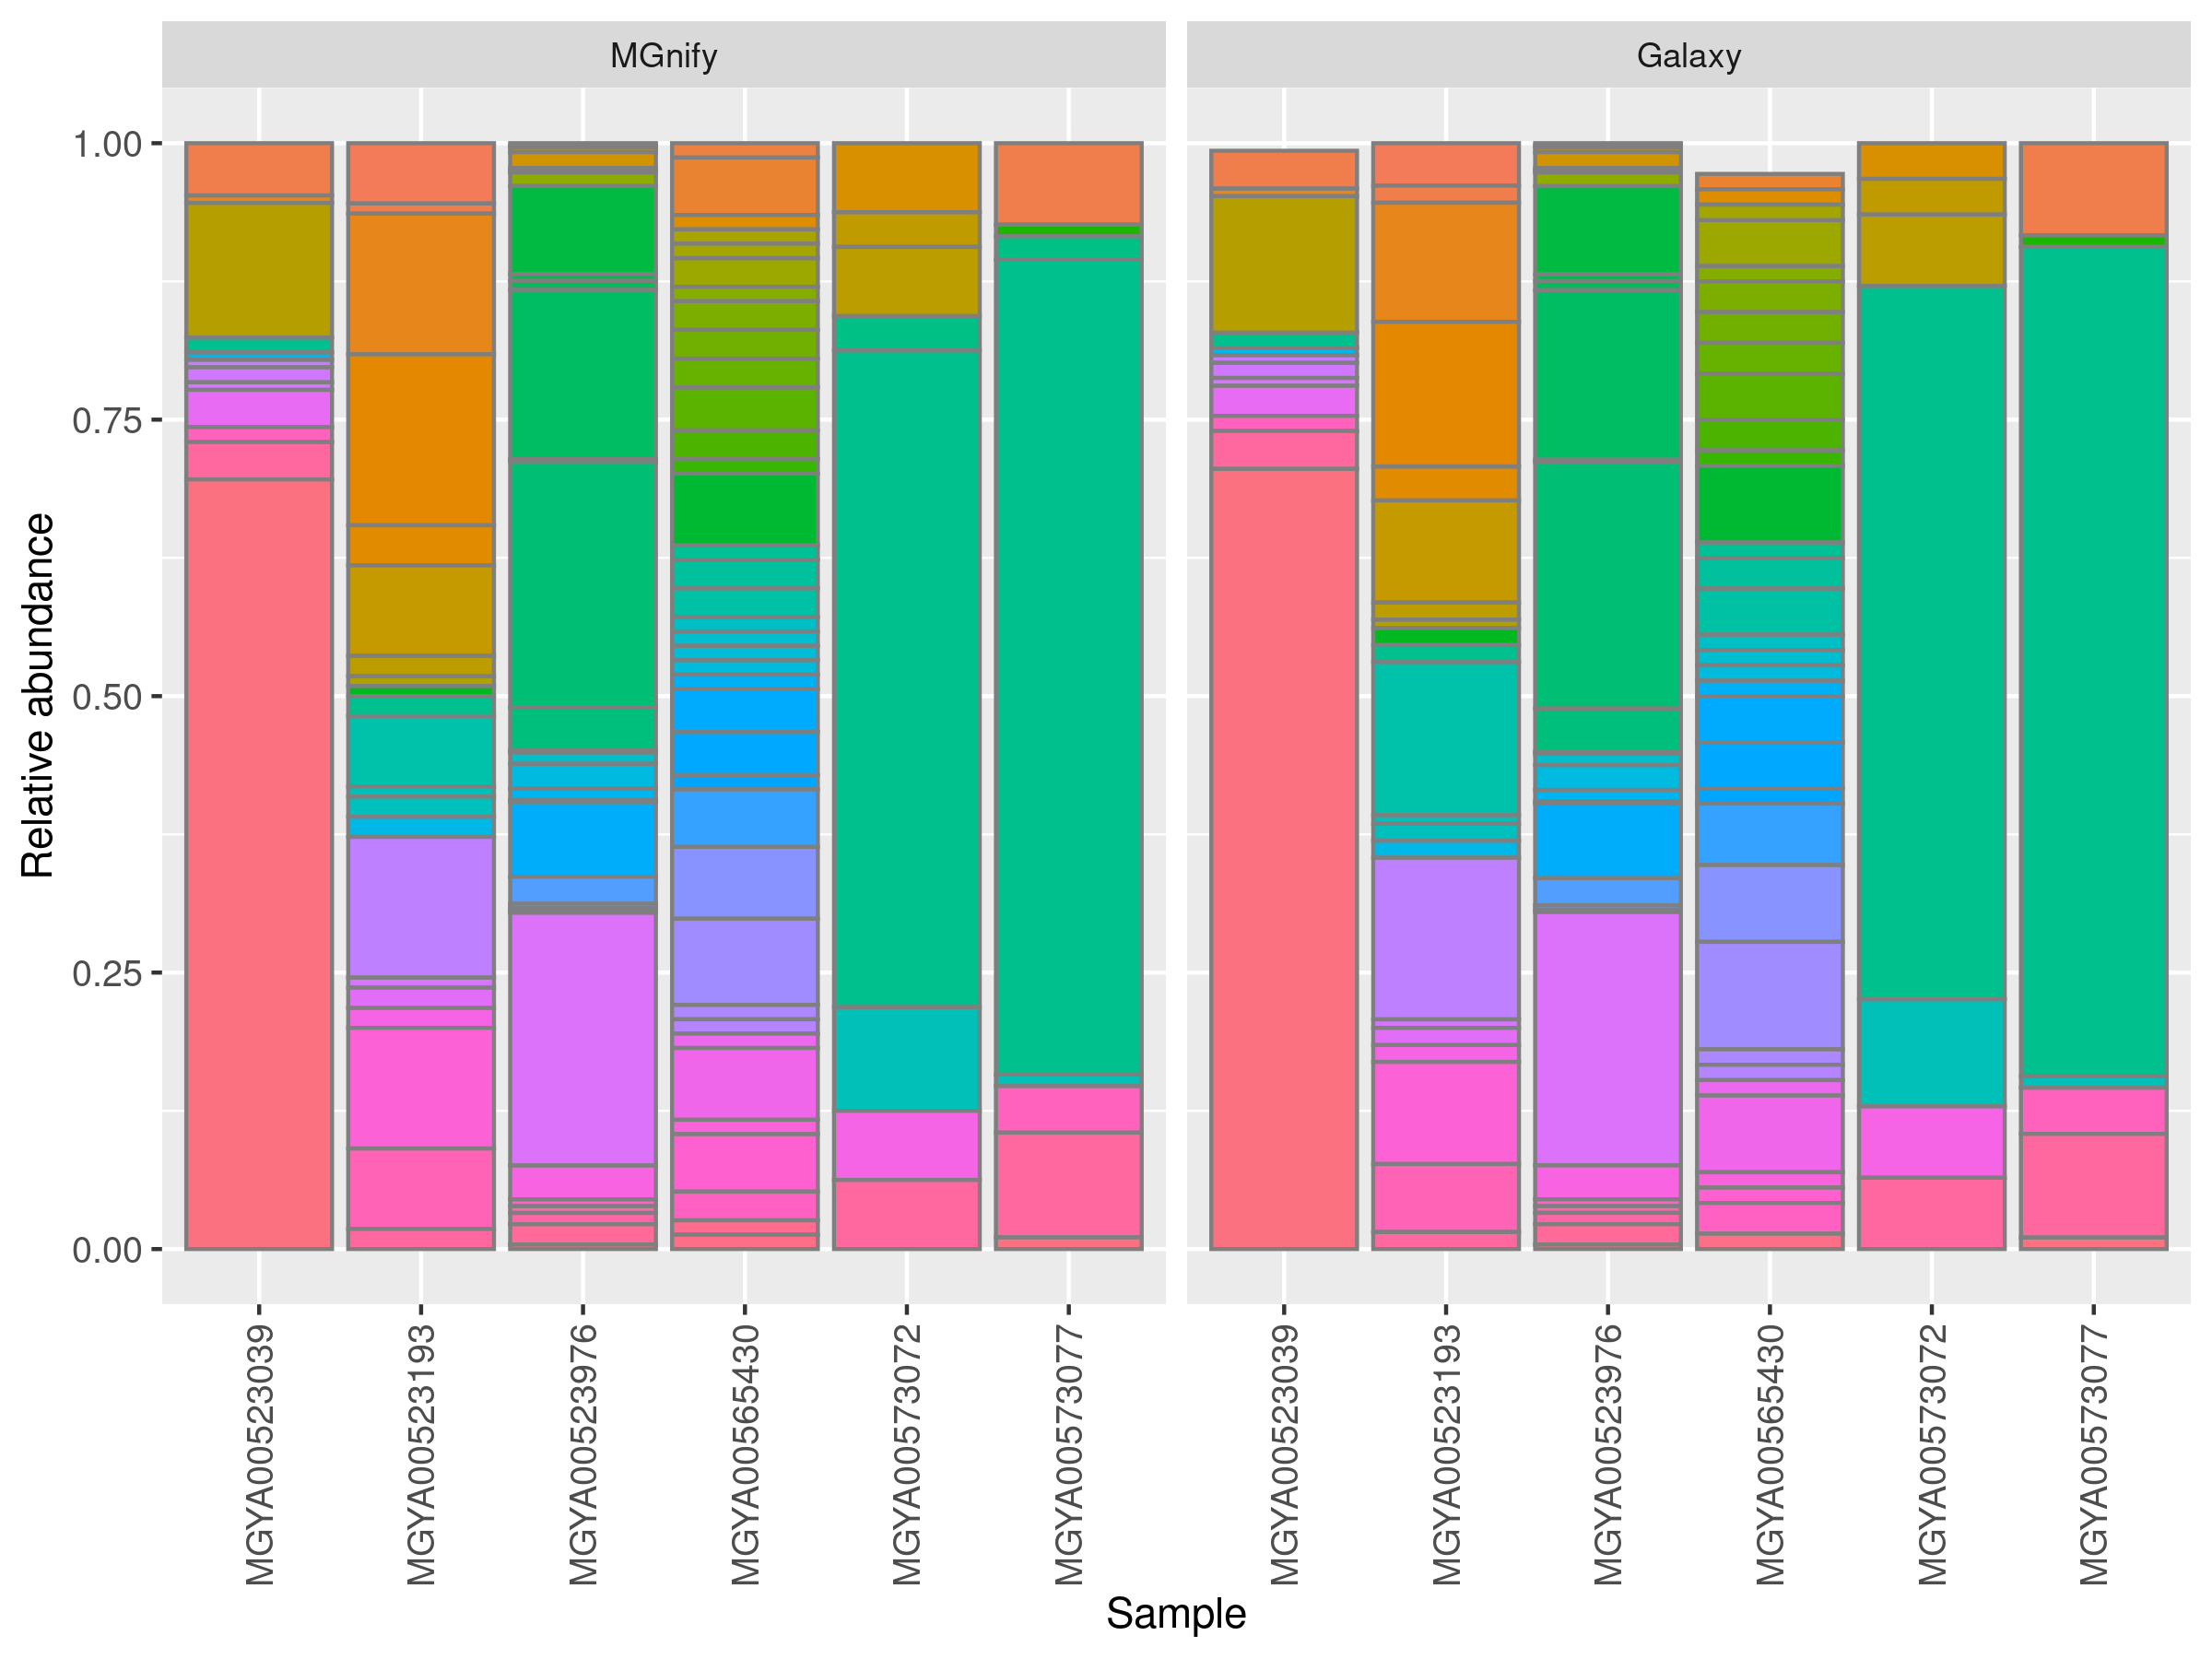
\includegraphics[scale=0.65]{figures/soil_abundace_level_s_mgnifyVSgalaxy.png} }}%
  \captionof{figure}[Differences of relative abundance between MGnify and Galaxy-ported pipeline at species rank for MGnify soil samples]{\textbf{Differences of relative abundance between MGnify and Galaxy-ported pipeline at species rank for MGnify soil samples}(\Cref{tab:soil-samples}). Species that were predicted by Galaxy but not present in the MGnify output are not shown. Some samples did not include any reads for the species rank. The plot legend can be found in the appendix (\Cref{fig:soil_abundace_level_s_mgnifyVSgalaxy_legend.png})} \label{fig:mgnify_soil_rel_abundace_s_level}%
\end{figure}

\begin{figure}[H]
  \centering
  \subfloat{{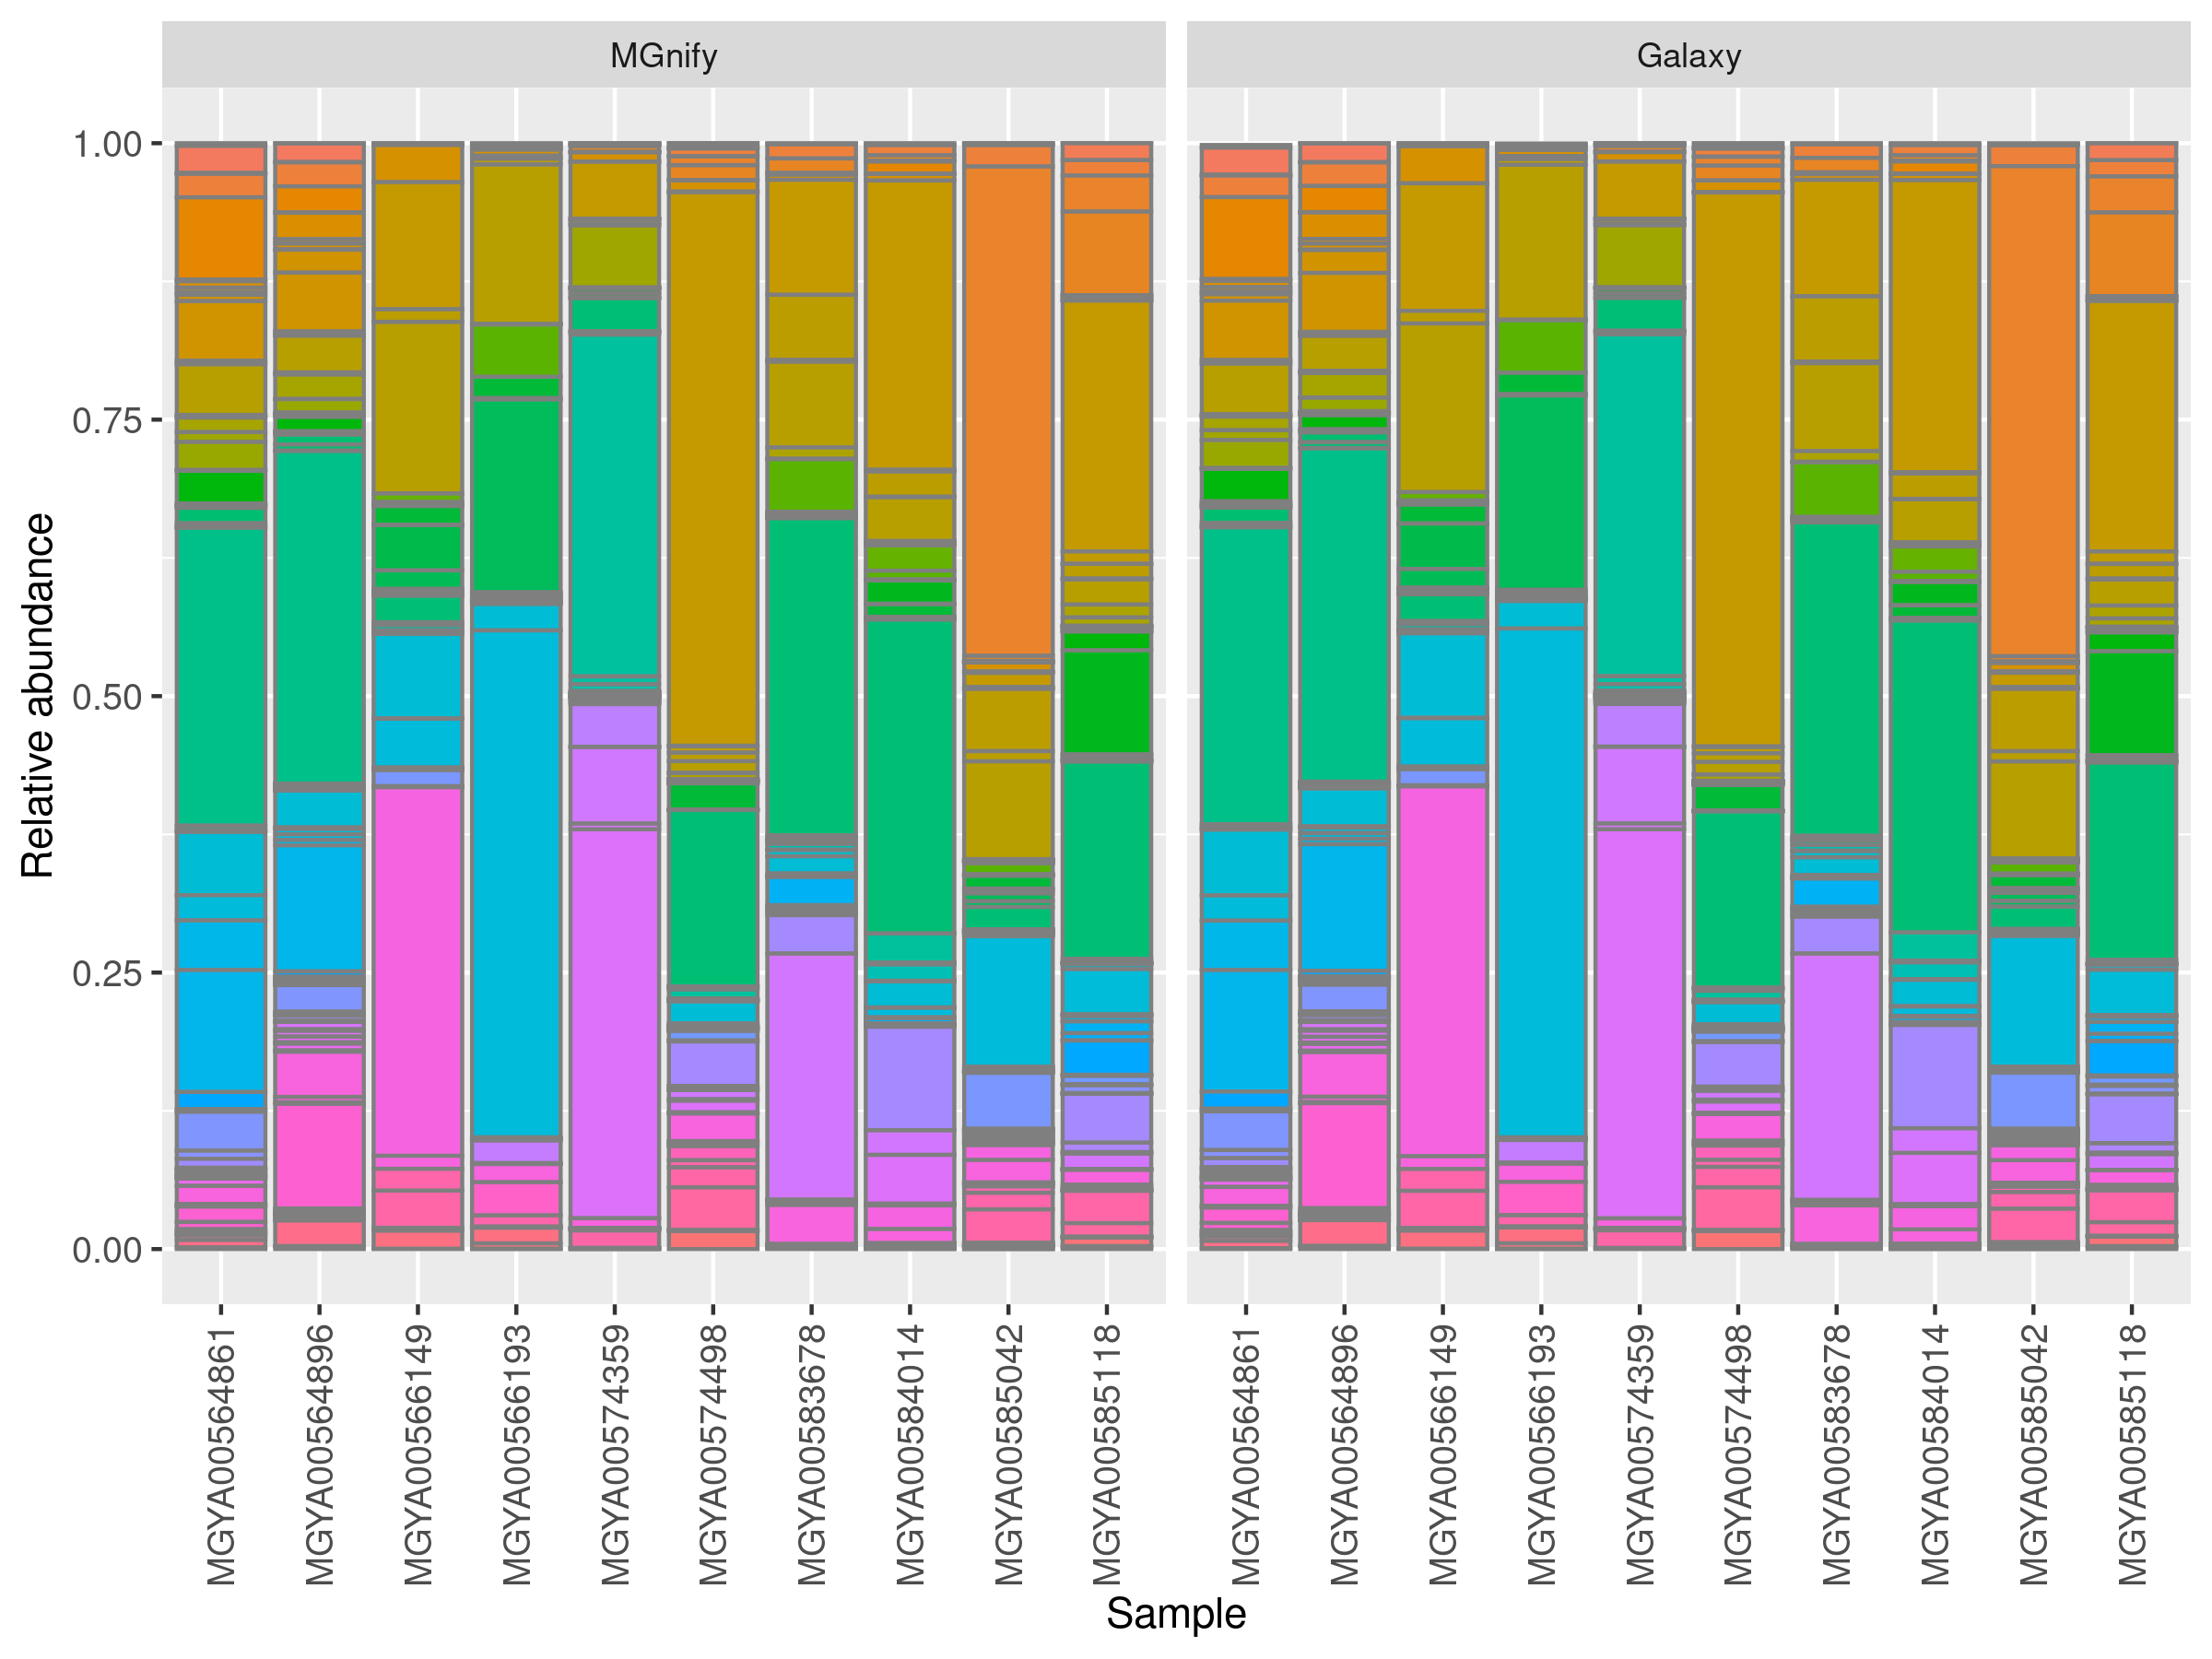
\includegraphics[scale=0.7]{figures/human_gut_abundance_level_g_mgnifyVSgalaxy.png} }}%
  \captionof{figure}[Differences of relative abundance between MGnify and Galaxy-ported pipeline at genus rank for MGnify human large intestine samples]{\textbf{Differences of relative abundance between MGnify and Galaxy-ported pipeline at genus rank for MGnify human large intestine samples}(\Cref{tab:human-gut-samples}). Genera that were predicted by Galaxy but not present in the MGnify output are not shown. The plot legend can be found in the appendix (\Cref{fig:human_gut_abundance_level_g_mgnifyVSgalaxy_legend.png})} \label{fig:mgnify_human_gut_rel_abundance_g_level}%
\end{figure}

\begin{figure}[H]
  \centering
  \subfloat{{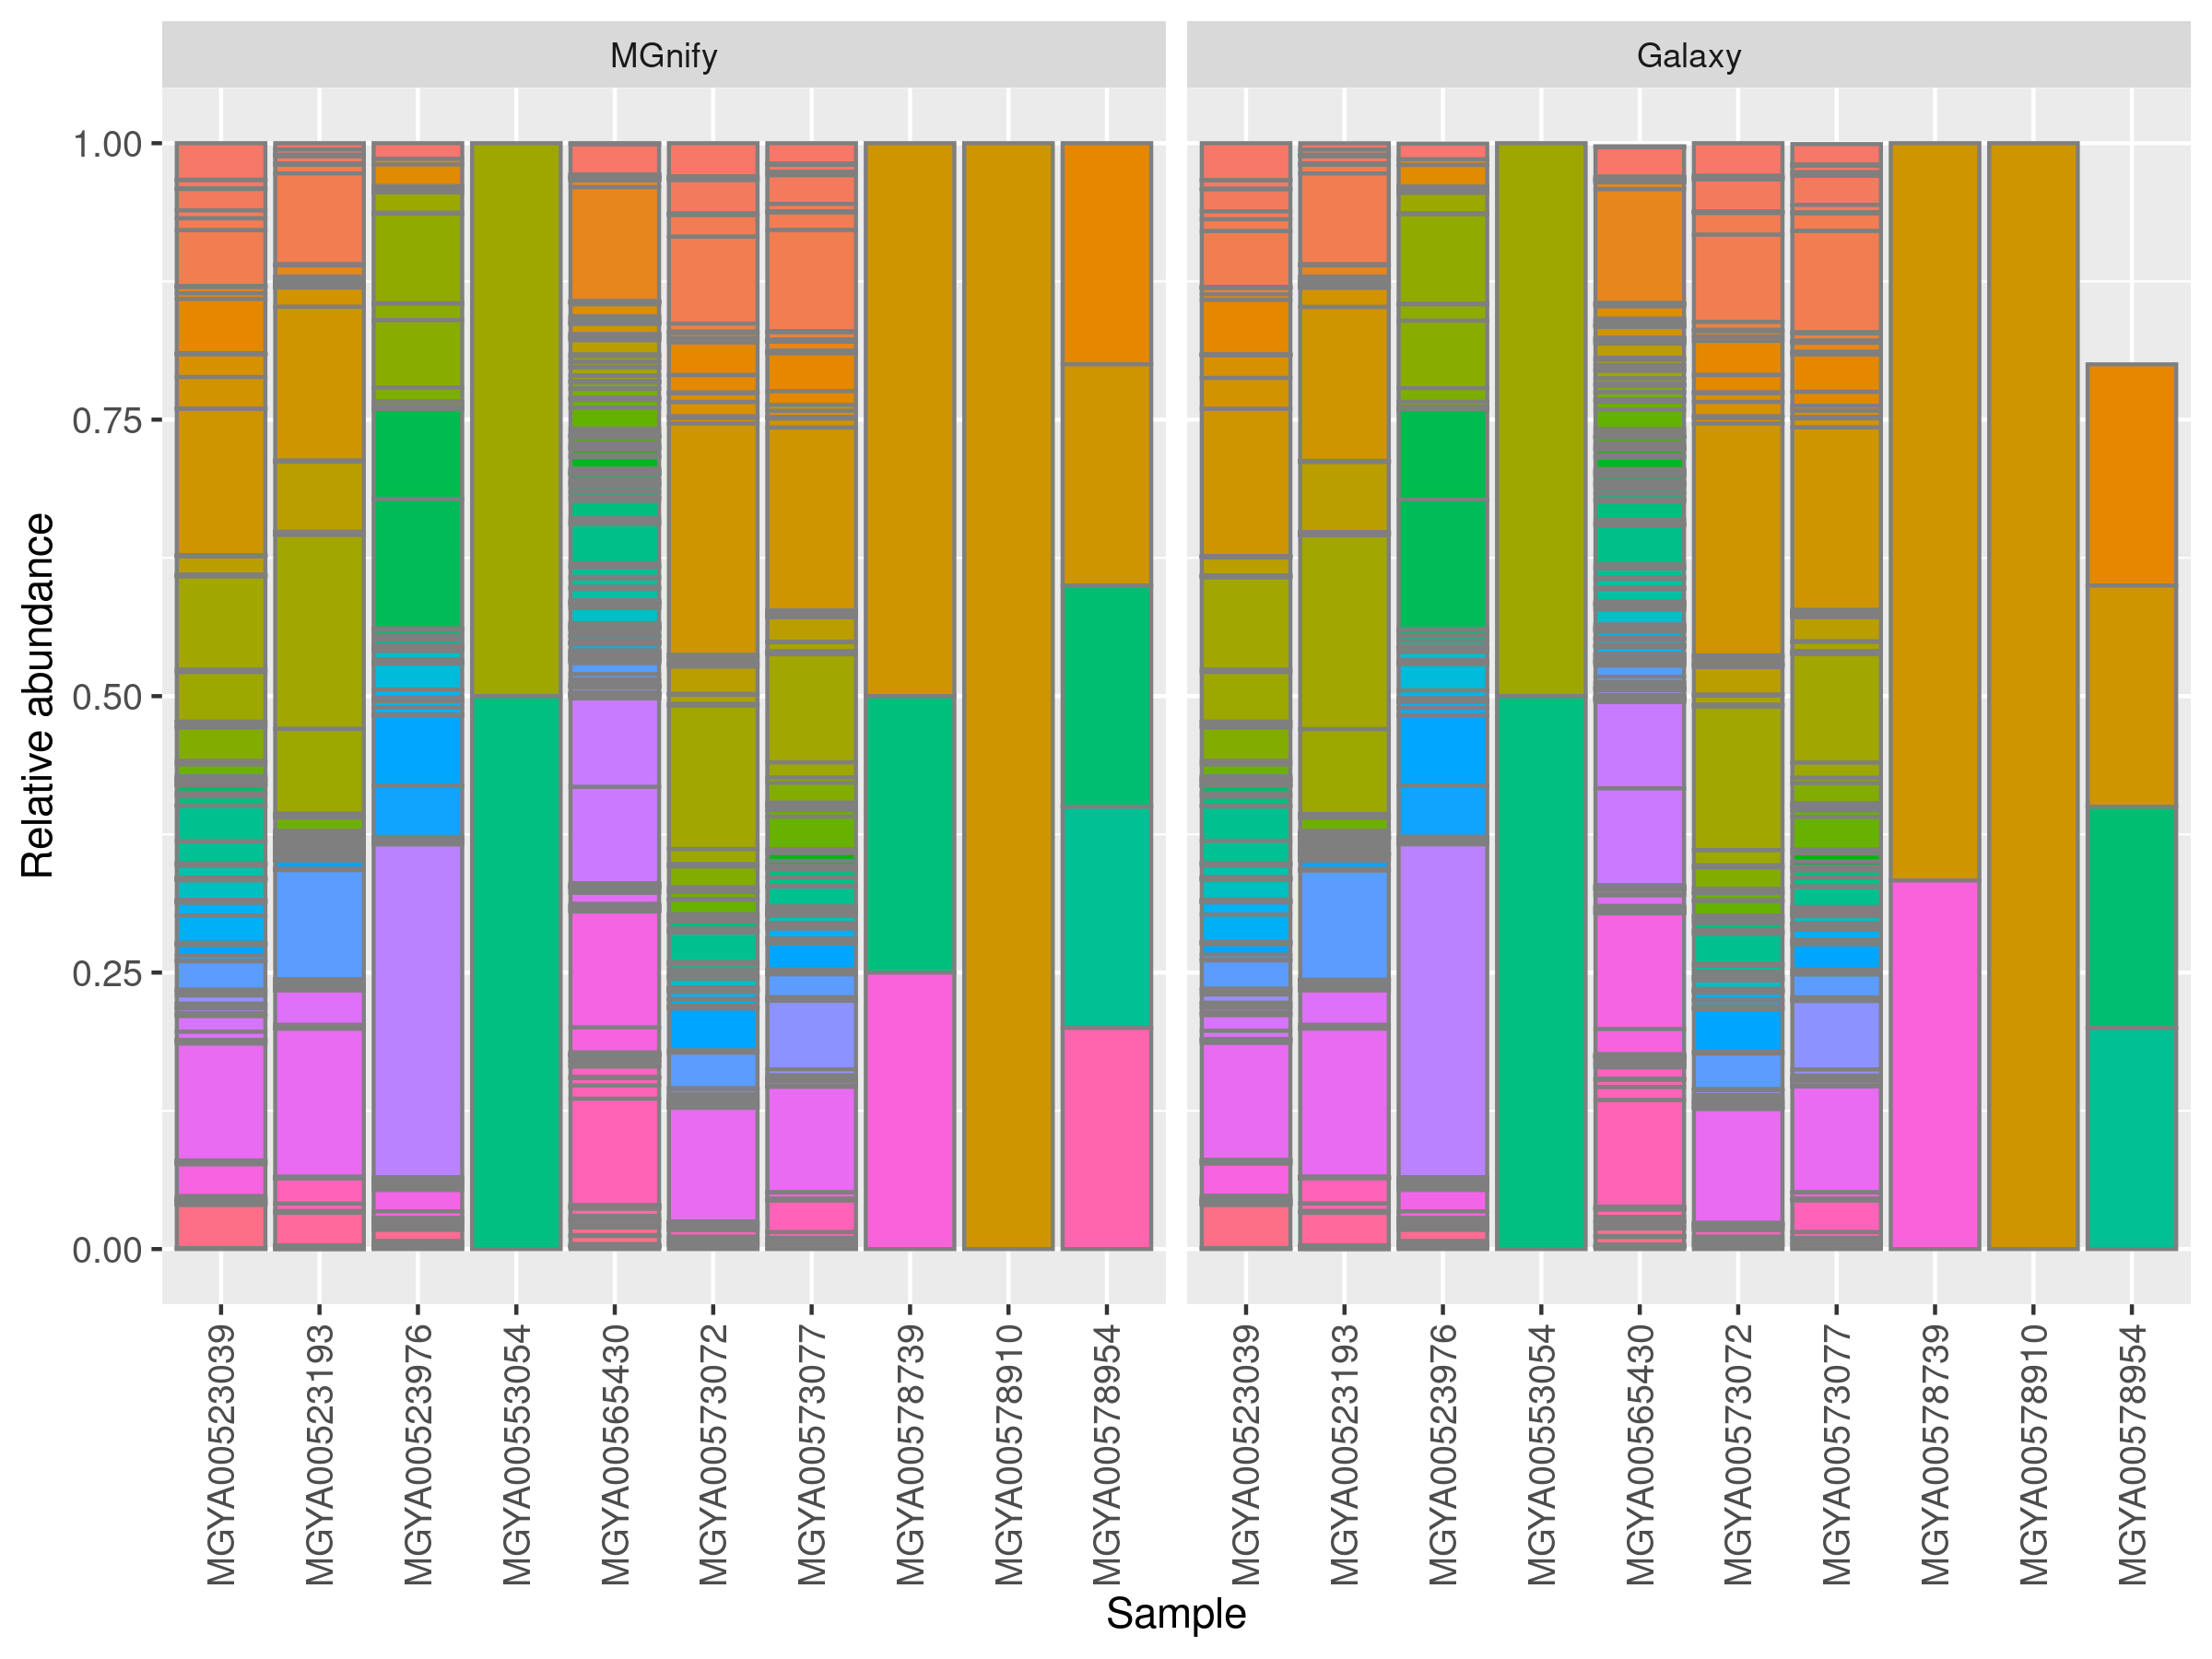
\includegraphics[scale=0.7]{figures/soil_abundance_level_g_mgnifyVSgalaxy.png} }}%
  \captionof{figure}[Differences of relative abundance between MGnify and Galaxy-ported pipeline at genus rank for MGnify soil samples]{\textbf{Differences of relative abundance between MGnify and Galaxy-ported pipeline at genus rank for MGnify soil samples}(\Cref{tab:soil-samples}). Genera that were predicted by Galaxy but not present in the MGnify output are not shown. The plot legend can be found in the appendix (\Cref{fig:soil_abundance_level_g_mgnifyVSgalaxy_legend.png})} \label{fig:mgnify_soil_rel_abundace_g_level}%
\end{figure}


\subsection{Benchmark of Kraken v2 against MGnify rRNA-prediction subworkflow}\label{subsec:mgnifyVSkraken2}
For the comparison between MGnify and Kraken v2, it was necessary to exclude the super kingdom and species ranks from MGnify results. Additionally, adjustments were made to the kingdom rank, to match the Kraken v2 taxonomic lineage.\\
The beta diversity plots (\Cref{fig:human_gut_plot_mgnifyVSkraken2.png,fig:soil_plot_mgnifyVSkraken2.png}) show overall high average dissimilarity values. Additionally, the average Jaccard distance values consistently exceeded the average Bray Curtis distance values. These substantial dissimilarities are also noticeable in the generated relative abundance plots for the genus rank (\Cref{fig:human_large_intestine_rel_abundance_mgnifyVSkraken2,fig:soil_rel_abundance_mgnifyVSkraken2}), where significant gaps in the Kraken v2 visual representation indicate a high relative abundance of detected taxa that are absent in MGnify results, especially within the soil samples.\\

\begin{figure}[H]
  \centering
  \hfill
  \subfloat{{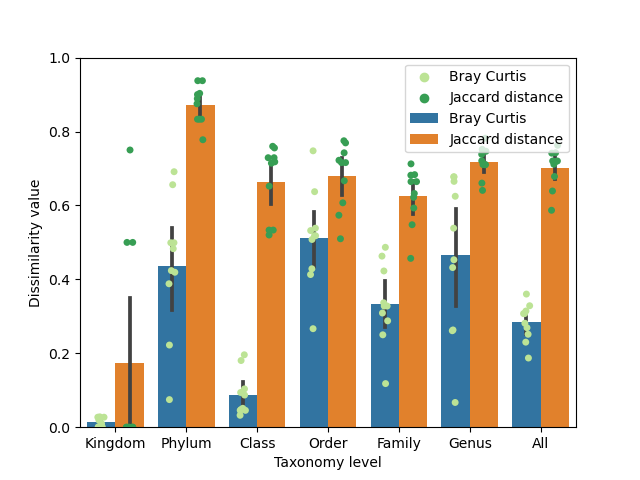
\includegraphics[scale=0.8]{figures/human_gut_plot_mgnifyVSkraken2.png} }}%
  \captionof{figure}[Beta diversity-based benchmark.Dissimilarity between MGnify and Kraken v2, for the MGnify human large intestine samples]{\textbf{Beta diversity-based benchmark}. Dissimilarity between MGnify and Kraken v2, for the MGnify human large intestine samples (\Cref{tab:human-gut-samples}) The term 'All' refers to all ranks combined. Bars represent the average dissimilarity values, while individual data points represent the values for each of the individual samples.} \label{fig:human_gut_plot_mgnifyVSkraken2.png}%
\end{figure}
\begin{figure}[H]
  \centering
  \hfill
  \subfloat{{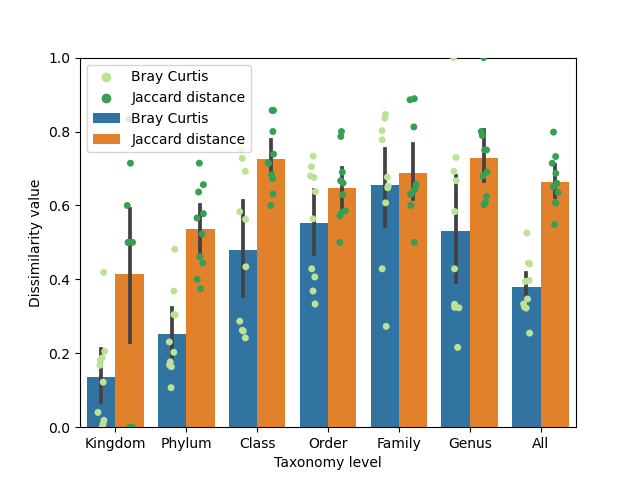
\includegraphics[scale=0.8]{figures/soil_plot_mgnifyVSkraken2.png} }}%
  \captionof{figure}[Beta diversity-based benchmark. Dissimilarity between MGnify and Kraken v2, for MGnify soil samples]{\textbf{Beta diversity-based benchmark}. Dissimilarity between MGnify and Kraken v2, for MGnify soil samples (\Cref{tab:soil-samples}). The term 'All' refers to all ranks combined. Bars represent the average dissimilarity values, while individual data points represent the values for each of the individual samples.}
  \label{fig:soil_plot_mgnifyVSkraken2.png}%
\end{figure}
\section{Mock samples benchmark}\label{sec:Mock samples}
The beta diversity benchmark for the mock samples is shown in \Cref{fig:mock_human_gut_beta_div_galaxy,fig:mock_soil_beta_div_kraken2}. Given that the taxonomic lineage for the mock sample and Kraken v2 starts at the kingdom rank and concludes at the genus rank, it was necessary to conduct the procedure of adjusting the Galaxy-port lineage, mentioned in \Cref{subsec:mgnifyVSkraken2}. Based on the two plots, it is evident that Galaxy-port (\Cref{fig:mock_human_gut_beta_div_galaxy}) outperformed Kraken v2 (\Cref{fig:mock_soil_beta_div_kraken2}). At each taxonomic rank, the Galaxy-port results displayed on average smaller Bray Curtis and Jaccard distances to the expected taxonomic composition compared to Kraken v2.\par

\begin{figure}[H]
  \centering
  \hfill
  \subfloat{{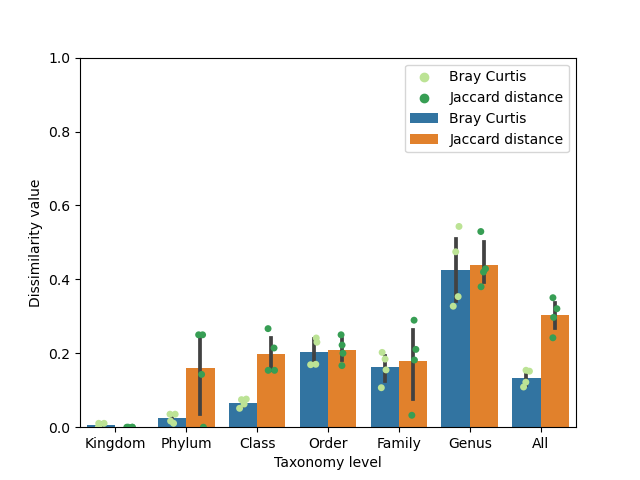
\includegraphics[scale=0.8]{figures/mock_beta_div_expectedVSgalaxy.png} }}%
  \captionof{figure}[Beta diversity-based benchmark. Dissimilarity between expected composition and Galaxy-ported subworkflow, for mock samples]{\textbf{Beta diversity-based benchmark}. Dissimilarity between expected composition and Galaxy-ported subworkflow, for the mock samples (\Cref{subsubsec:mock_samples}). The term 'All' refers to all ranks combined. Bars represent the average dissimilarity values, while individual data points represent the values for each of the individual samples.} \label{fig:mock_human_gut_beta_div_galaxy}%
\end{figure}

\begin{figure}[H]
  \centering
  \hfill
  \subfloat{{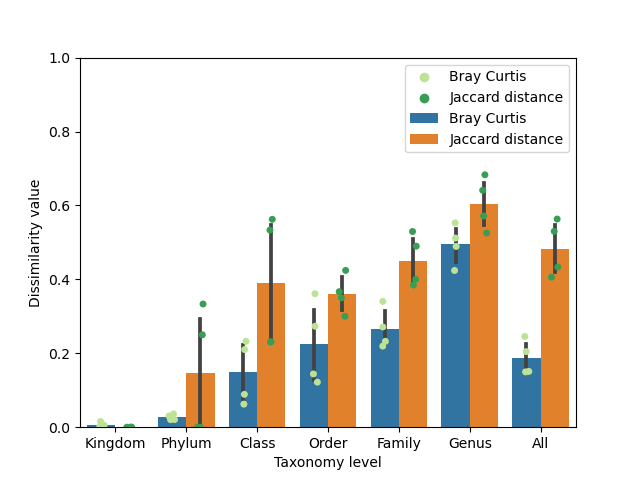
\includegraphics[scale=0.8]{figures/mock_beta_div_expectedVSkraken2.png} }}%
  \captionof{figure}[Beta diversity-based benchmark. Dissimilarity between expected composition and Kraken v2 for mock samples]{\textbf{Beta diversity-based benchmark}. Dissimilarity between expected composition and Kraken v2, for the mock samples (\Cref{subsubsec:mock_samples}). The term 'All' refers to all ranks combined.Bars represent the average dissimilarity values, while individual data points represent the values for each of the individual samples.} \label{fig:mock_soil_beta_div_kraken2}%
\end{figure}

Regarding the generated genus rank relative abundance plot, taxa in the output of Galaxy-ported and Kraken v2 that are differed from the expected taxonomic composition were excluded. The plot of the relative abundance at the genus rank supports the superior performance of Galaxy-port over Kraken v2. The Galaxy visual representation exhibits smaller gaps in comparison to Kraken v2, which means Kraken v2 had higher relative abundance for unexpected taxa. 


\begin{figure}[H]
  \centering
  \subfloat{{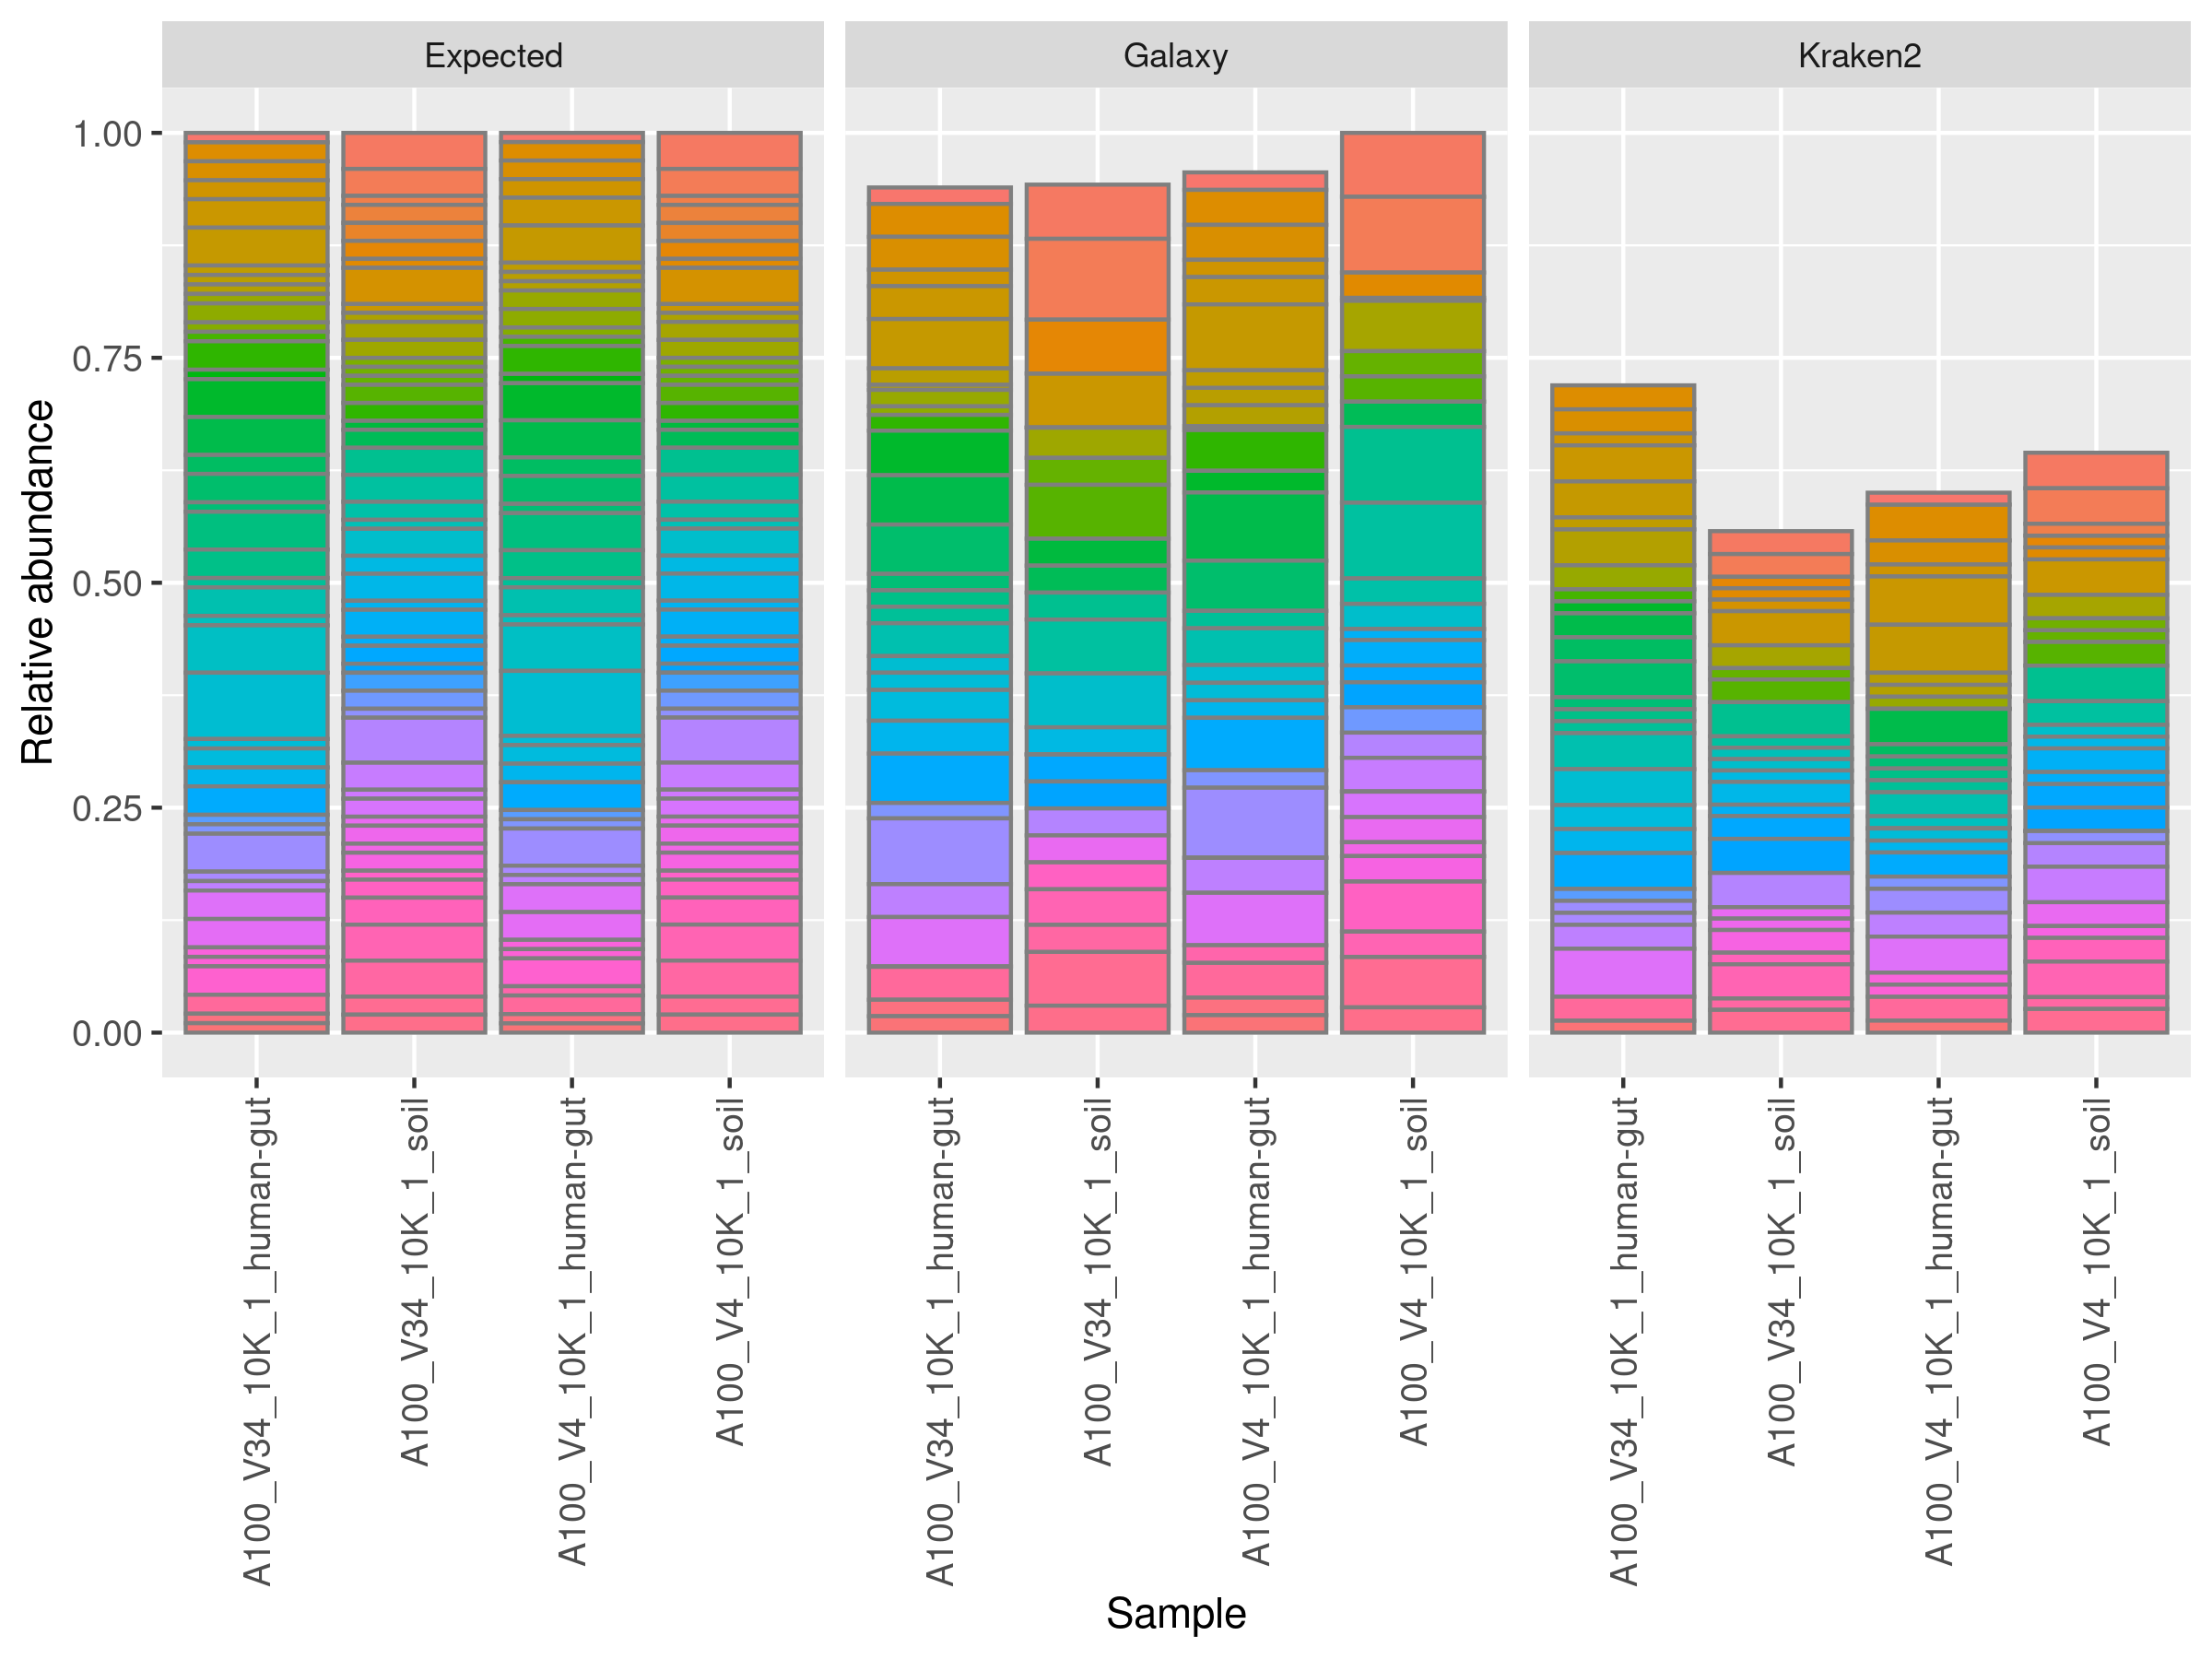
\includegraphics[scale=0.65]{figures/mock_samples_abundance_level_g.png} }}%
  \captionof{figure}[Differences of relative abundance between expected composition, Galaxy-ported subworkflow, and Kraken v2 at genus rank for mock samples]{\textbf{Differences of relative abundance between expected composition, Galaxy-ported subworkflow, and Kraken v2 at genus rank for the mock samples}(\Cref{subsubsec:mock_samples}). Genera that were predicted by Galaxy and Kraken v2 but not present in the expected composition are not shown. The plot legend can be found in the appendix (\Cref{fig:mock_rel_abundance_level_g_legend}).} \label{fig:mock_rel_abundance}%
\end{figure}
\section{Differences in MAPseq output}\label{results_MAPseq_inconsistency}
During the development of the ported pipeline, the tool MAPseq was discovered to be inconsistent. Executed several times using the identical command, configuration, input, and database files, the output would occasionally vary.\par
To demonstrate this behaviour MAPseq was executed ten times, in conjunction with the MGnify-compatible database files and the SSU FASTA file from analysis MGYA00578954 (\Cref{tab:soil-samples}) as an input. Subsequently, each output was compared to the MGnify output using beta diversity metrics, specifically Bray Curtis distance and Jaccard distance, as previously described in \Cref{sec:Benchmark}.

\begin{figure}[H]
  \centering
  \hfill
  \subfloat{{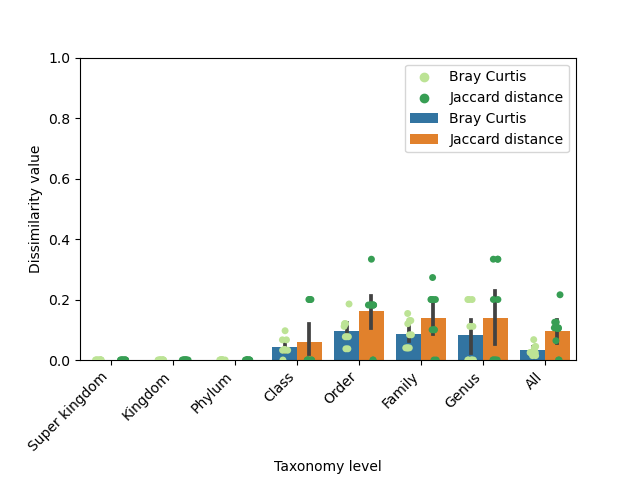
\includegraphics[scale=0.8]{figures/mapseq_test_beta_div_plot.png} }}%
  \captionof{figure}[Beta diversity-based benchmark. Dissimilarity between MGnify and MAPseq, for MAPseq inconsistency demonstration]{\textbf{Beta diversity-based benchmark}. Dissimilarity between MGnify and MAPseq. Executed ten times using identical configuration and the same sample from analysis MGYA00578954 (\Cref{tab:soil-samples}) to demonstrate MAPseq inconsistency. The term 'All' refers to all ranks combined. Species rank was excluded, due to taxa absence at this rank. Bars represent the average dissimilarity values, while individual data points represent the values for each of the ten different runs.} \label{fig:mapseq_test_beta_div_plot.png}%
\end{figure}

The dissimilarity values for MAPseq using identical input multiple times are shown in \Cref{fig:mapseq_test_beta_div_plot.png}. Neither of the execution delivered taxa in the species rank. The ranks super kingdom, kingdom, and phylum consisted of identical results. The average dissimilarity values were variable between the ranks class and genus, with the rank order having the highest average distance values for both Bray Curtis and Jaccard metrics.
\chapter{Discussion and outlook}\label{chap:Discussion}
In this thesis, the rRNA-prediction subworkflow from the MGnify amplicon pipeline v5.0 was successfully ported to Galaxy. The process included integration or substitution of absent tools and reconstruction of the subworkflow on Galaxy, which resulted in an available, working subworkflow within the Galaxy platform. The link to Galaxy-ported rRNA-prediction subworkflow can be found in \Cref{appendix_galaxy_workflows}.\par
The beta diversity-based benchmark between MGnify and Galaxy-port, performed on samples from previous MGnify analyses, showed overall high similarity. The two beta diversity metrics, employed during this thesis, indicated low dissimilarity values for higher taxonomic ranks. The Jaccard distance values were consistently higher than the Bray Curtis distance values, which resulted from minority taxa (taxa with low abundance) being present in MGnify results and absent in Galaxy-port results, or vice versa.\\
The dissimilarities could be attributed to the inconsistency of the tool MAPseq. The taxonomic classifier, MAPseq, appeared to have a non-deterministic algorithm, which lead to slightly inconsistent outputs. MAPseq, when tested multiple times using identical command, configuration, input, and database files, occasionally delivered slightly different outputs. This issue of MAPseq was brought to the attention of both the MGnify team and the MAPseq developers, seeking clarification.\par
The beta diversity benchmark between MGnify and Kraken v2, conducted on samples from previous MGnify analyses, delivered notably high dissimilarity values. Several factors might have contributed to the high dissimilarity. Firstly, Kraken v2 used a 16S SILVA database, while the MGnify samples originate from SSU analyses. Since 16S and 18S SSU analyses are not distinctly categorized in MGnify, it cannot not be ruled out that the MGnify samples include 18S SSUs as well. Secondly, Kraken v2 used a newer SILVA database version (v138) compared to MGnify (SILVA v132). The choice to use Kraken v2 in conjunction with SILVA 16S v138 was driven by its availability on the Galaxy platform, as SILVA 16S v132 was not accessible. Lastly, the SILVA v138 database files, compatible for use with MGnify are currently unavailable. According to SILVA these files are unlikely to be available before 2025.\par
A more informative comparison between Kraken v2 and the rRNA-prediction subworkflow, was conducted on 16S mock samples. The benchmark compared the results of the Galaxy-ported rRNA-prediction and Kraken v2 against the expected composition of the mock samples. The choice of 16S mock samples provided a more robust comparison, as Kraken v2 used the 16S SILVA database. Despite Kraken v2 using a newer SILVA database version (v138) in comparison to the Galaxy-ported version (SILVA v132), the rRNA-prediction subworkflow on Galaxy consistently outperformed Kraken v2. The Galaxy-ported rRNA-prediction subworkflow yielded lower dissimilarity values than Kraken v2, indicating that it was closer to the expected composition of the mock samples. This observation is additionally supported by the generated relative abundance plot for the genus rank, which indicated higher abundances of false-positive taxa for Kraken v2 in comparison to the Galaxy-ported rRNA-prediction subworkfow.\par
In summary, the integration and construction of the rRNA-prediction subworkflow, part of MGnify amplicon pipeline v5.0, within Galaxy was executed successfully. The Benchmark, comparing the Galaxy-ported version against its original counterpart, demonstrated good agreement between results. However, slight differences were detected, towards lower taxonomic ranks. Regarding both MGnify and Galaxy-ported results, the super kingdom and kingdom ranks exhibited identical taxa presence and nearly identical taxa abundance.\\
While the recent study by Odom \emph{et al.} reported a strong performance of Kraken v2~\cite{odom_metagenomic_2023} for amplicon prediction, the rRNA-prediction subworkflow consistently outperformed Kraken v2.\\
The availability of the workflow on Galaxy facilitates interoperability, shareability, integration with MGnify Jupyter Notebooks, downstream analysis using machine learning and differential abundance analysis. Additionally, Galaxy facilitates exchange and modification of specific tools. However, results reproducibility and comparability are limited due to the non-deterministic algorithm of MAPseq.\par
In future work, the Galaxy-ported rRNA-prediction subworkflow can be further evaluated using samples from LSU MGnify analyses. Since rRNA-prediction is a common subworkflow across all three MGnify pipelines amplicon, raw metagenomic reads, and assembly, its availability on Galaxy supports future work on these pipelines. Ongoing work is dedicated to port the quality control and ITS subworkflows, of the amplicon pipeline, which will soon make the entire pipeline available on Galaxy.
\appendix
\chapter{Appendix}\label{appendix}
\section{Additional figures and tables}\label{appendix_further_figures}

\begin{figure}[H]
  \centering
  \subfloat{{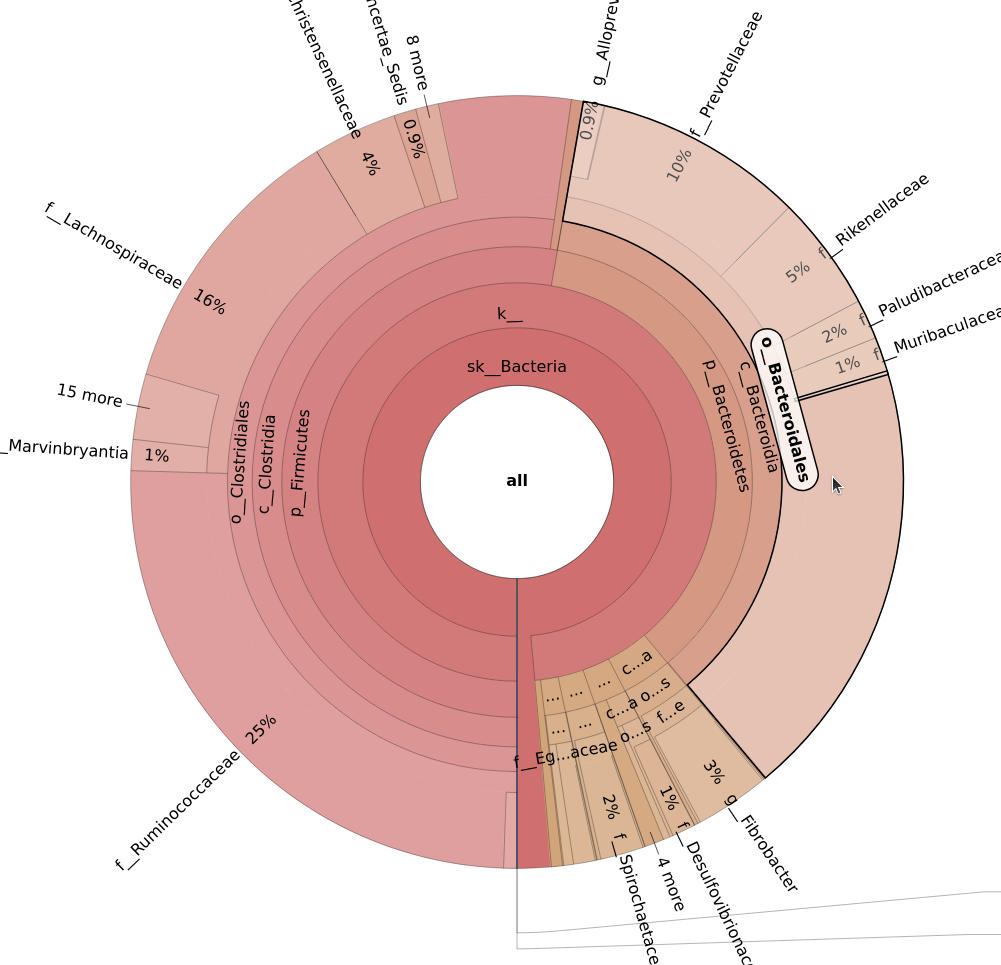
\includegraphics[scale=0.4]{figures/krona_example.png} }}%
  \captionof{figure}[A Krona pie chart example]{\textbf{A Krona pie chart example}. The chart visualizes the taxonomic abundance of the sample ERS4804749 (\Cref{tab:human-gut-samples}).} \label{fig:krona_example}%
\end{figure}

\begin{table}
    \centering
    \begin{tabular}{|c|c|c|}
        \hline
        Species & MGnify & Galaxy\\
        \hline \hline
        Blautia\textunderscore massiliensis & 23 & 16\\
        \hline
        Clostridiales\textunderscore bacterium\textunderscore CHKCI006 & 1 & 1\\
        \hline
        \textbf{Coprococcus\textunderscore catus} & \textbf{1} & \textbf{0}\\
        \hline
        \textbf{Dorea\textunderscore formicigenerans} & \textbf{1} & \textbf{0}\\
        \hline
        Dubosiella\textunderscore newyorkensis & 1 & 1\\
        \hline
        Firmicutes\textunderscore bacterium\textunderscore M10-2 & 1 & 1\\
        \hline
        \textbf{[Clostridium]\textunderscore scindens} & \textbf{1} & \textbf{0}\\
        \hline
        \textbf{Anaerostipes\textunderscore hadrus} & \textbf{0} & \textbf{1}\\
        \hline
        \textbf{Ruminococcus\textunderscore sp} & \textbf{0} & \textbf{1}\\
        \hline
    \end{tabular}
    \caption[Species abundance table for analysis MGYA00566149]{\textbf{Species abundance table for analysis MGYA00566149}. An example of present/absent taxa (see bold marked rows) causing a high Jaccard distance value.}
    \label{jaccard_example}
\end{table}


\subsection{Relative abundance figures}\label{appendix_rel_abundance_figures}

\begin{figure}[H]
  \centering
  \subfloat{{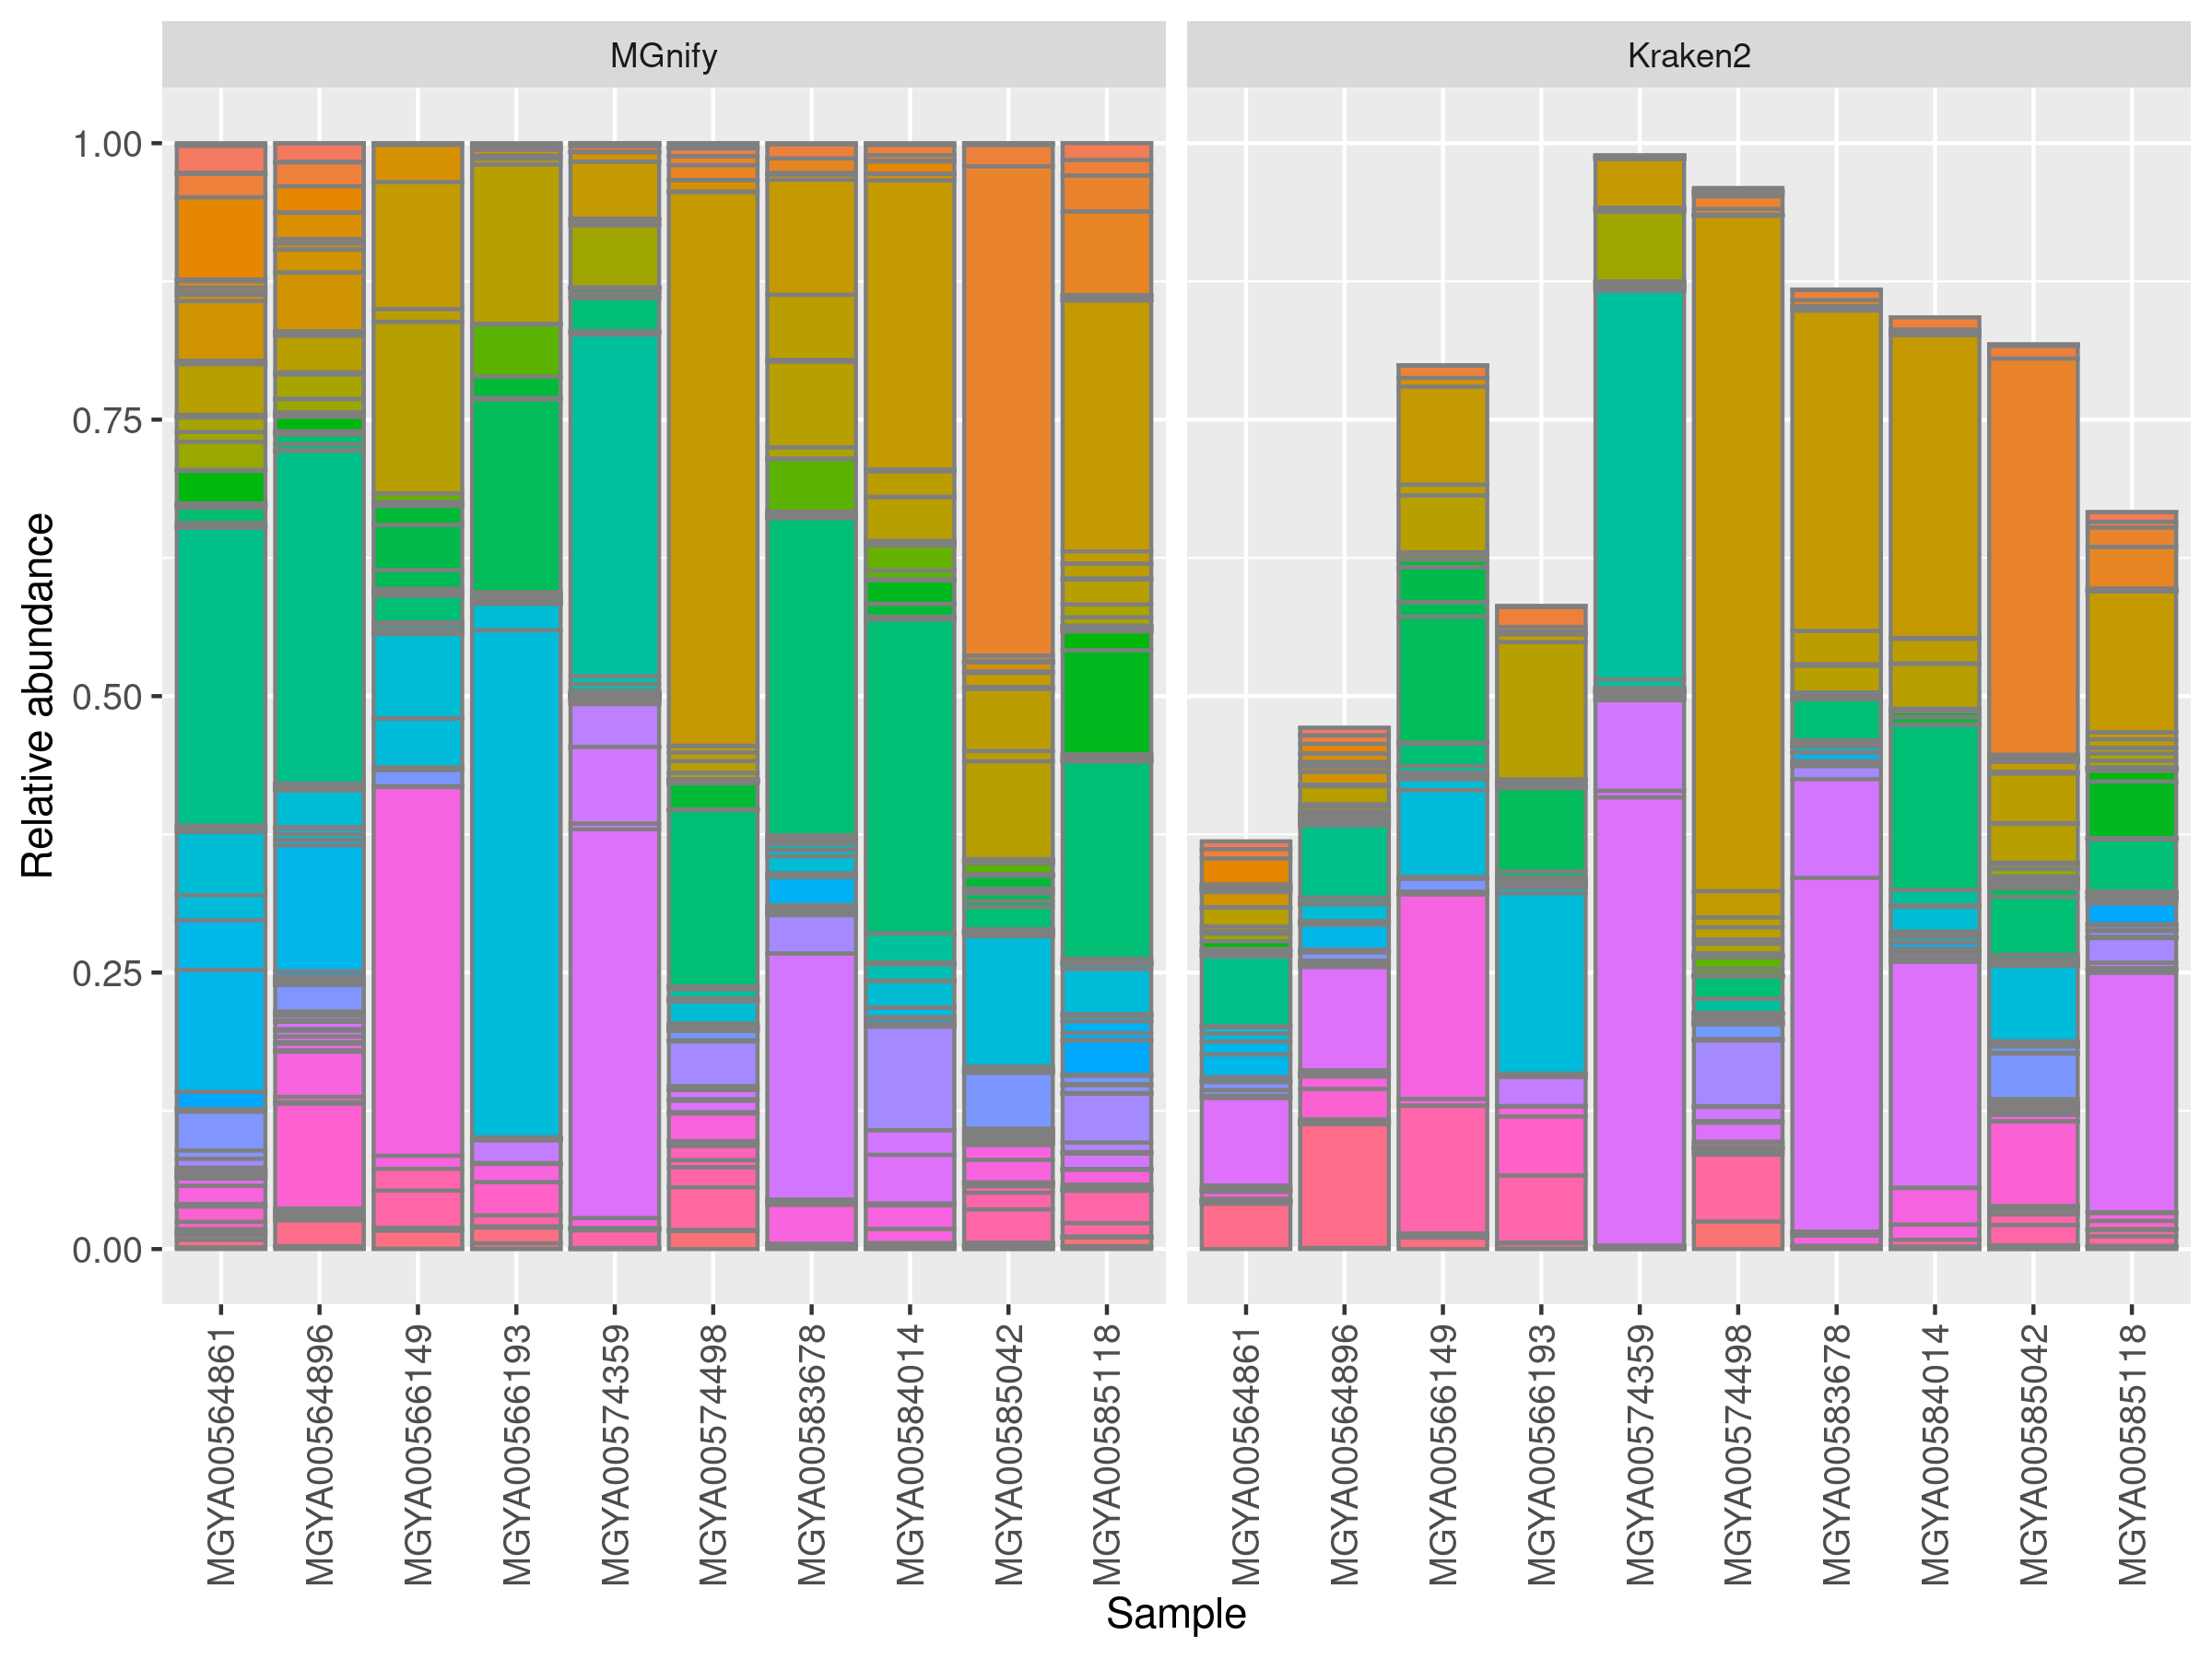
\includegraphics[scale=0.7]{figures/human_gut_abundance_level_g_mgnifyVSKraken.png} }}%
  \captionof{figure}[Differences of relative abundance between MGnify pipeline and Kraken v2 at genus rank for MGnify human large intestine samples]{\textbf{Differences of relative abundance between MGnify pipeline and Kraken v2 at genus rank for MGnify human large intestine samples} (\Cref{tab:human-gut-samples}). Genera that were predicted by Kraken v2 but not present in the MGnify output are not shown. The plot legend can be found in the appendix (\Cref{fig:human_gut_abundance_level_g_mgnifyVSKraken_legend.png})} \label{fig:human_large_intestine_rel_abundance_mgnifyVSkraken2}%
\end{figure}

\begin{figure}[H]
  \centering
  \subfloat{{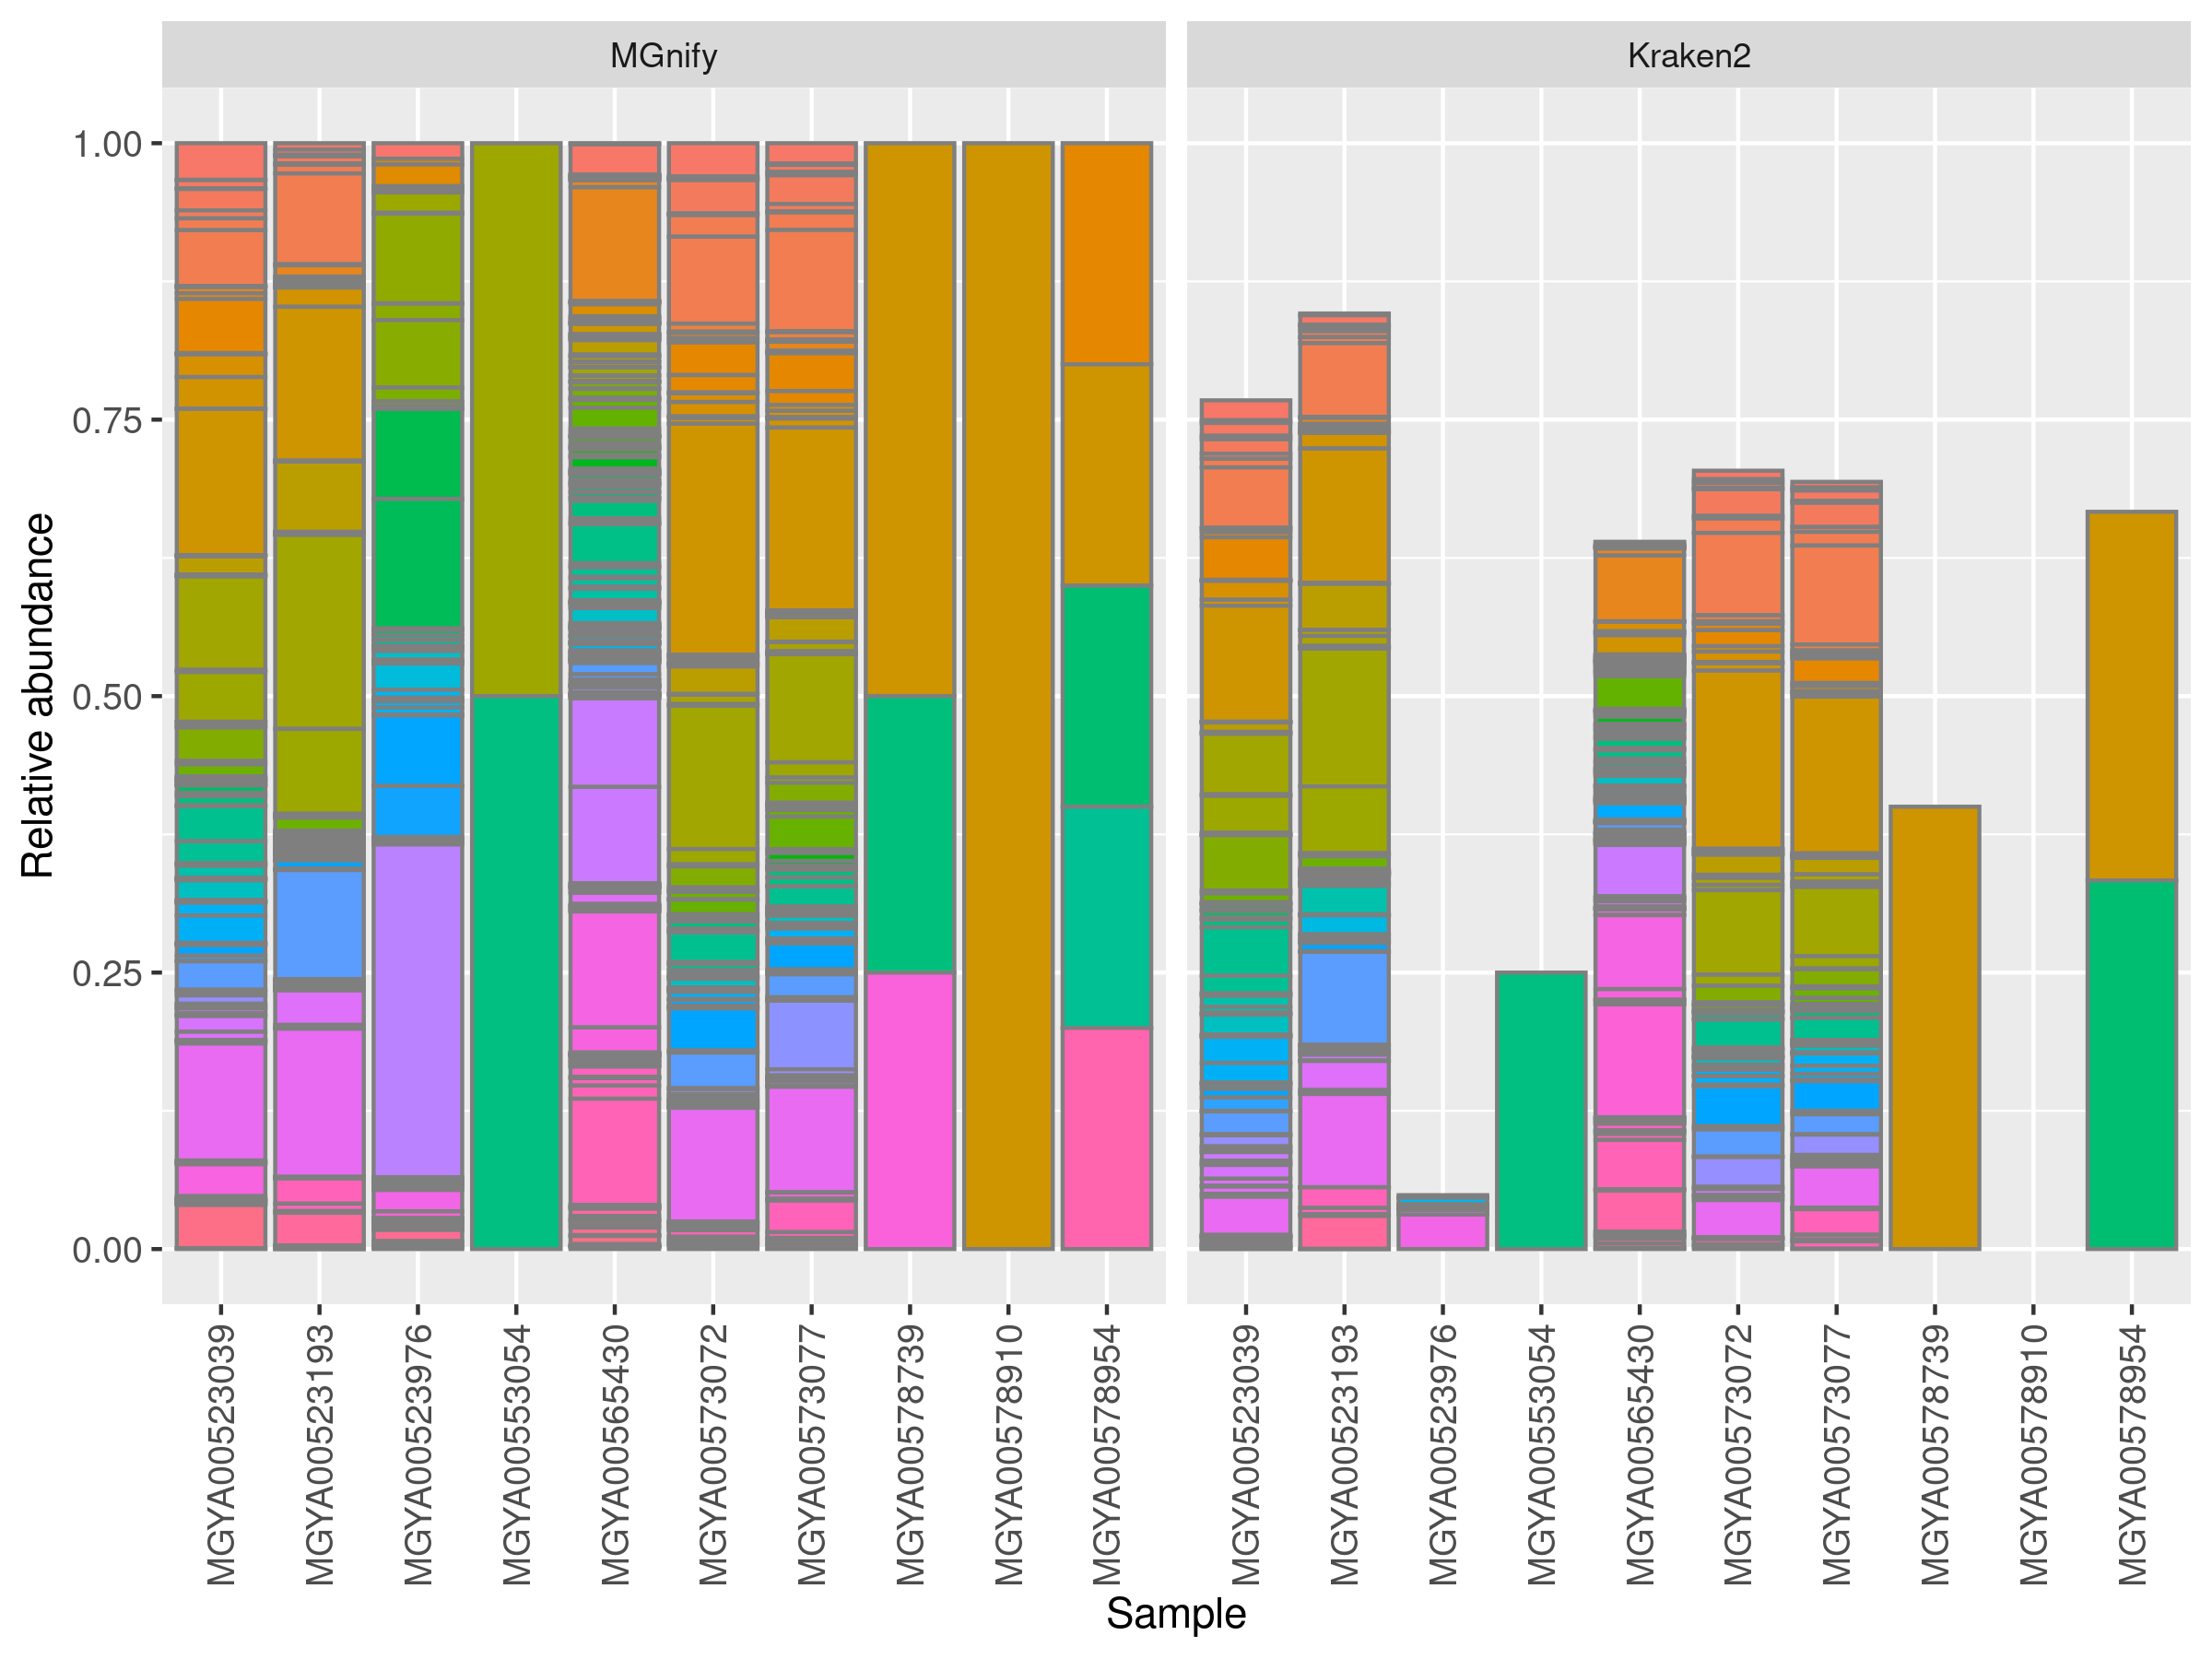
\includegraphics[scale=0.7]{figures/soil_abundance_level_g_mgnifyVSkraken2.png} }}%
  \captionof{figure}[Differences of relative abundance between MGnify pipeline and Kraken v2 at genus rank for MGnify soil samples]{\textbf{Differences of relative abundance between MGnify pipeline and Kraken v2 at genus rank for MGnify soil sample} (\Cref{tab:soil-samples}). Genera that were predicted by Kraken v2 but not present in the MGnify output are not shown. The plot legend can be found in the appendix (\Cref{fig:soil_abundance_level_g_mgnifyVSkraken2_legend.png})} \label{fig:soil_rel_abundance_mgnifyVSkraken2}%
\end{figure}
\newpage

\begin{landscape}
\subsection{Figure legends}\label{appendix_legends}
\vfill
\begin{figure}[H]
  \centering
  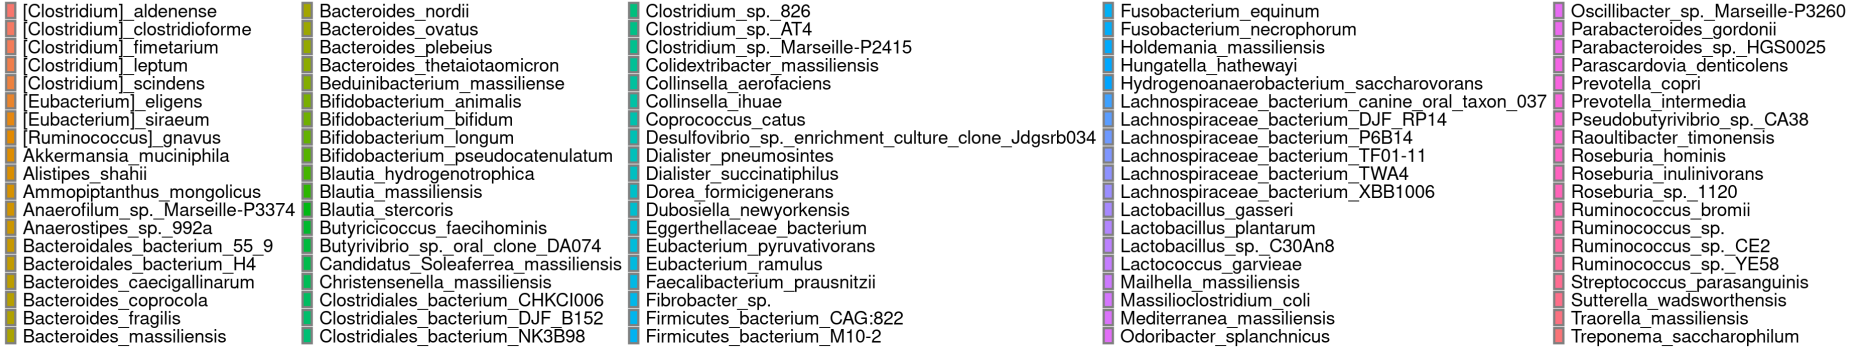
\includegraphics[width=1\linewidth, height=3\textheight, keepaspectratio]{figures/human_gut_abundance_level_s_mgnifyVSgalaxy_legend.png}
  \captionof{figure}[Legend of MGnify human large intestine samples relative abundance plot, comparing MGnify and Galaxy-port at species rank]{\textbf{Legend of MGnify human large intestine samples relative abundance plot, comparing MGnify and Galaxy-port at species rank}.} \label{fig:human_gut_abundance_level_s_mgnifyVSgalaxy_legend.png}%
\end{figure}
\vfill

\begin{figure}
  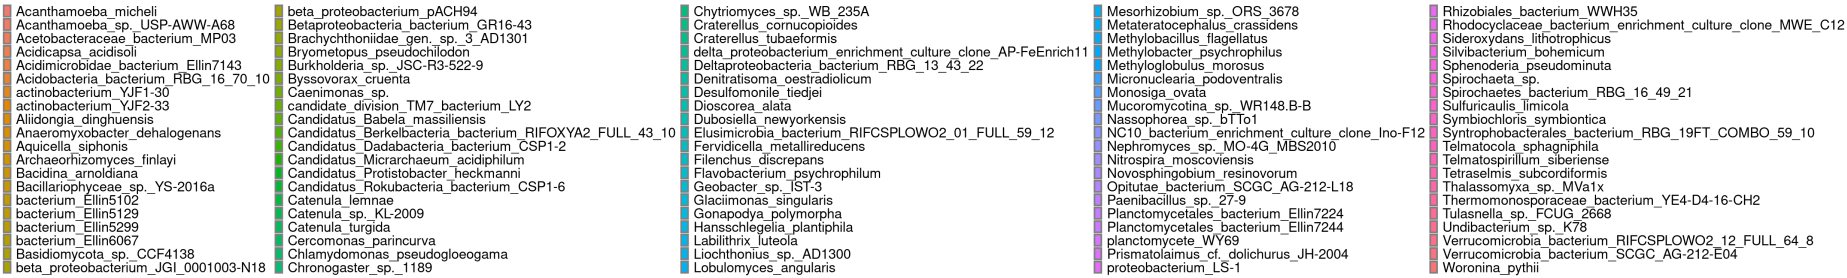
\includegraphics[width=1.1\linewidth, height=0.2\textheight]{figures/soil_abundace_level_s_mgnifyVSgalaxy_legend.png}
  \captionof{figure}[Legend of MGnify soil samples relative abundance plot, comparing MGnify and Galaxy-port at species rank]{\textbf{Legend of MGnify soil samples relative abundance plot, comparing MGnify and Galaxy-port at species rank}.} \label{fig:soil_abundace_level_s_mgnifyVSgalaxy_legend.png}%
\end{figure}
\end{landscape}


\begin{figure}[H]
  \centering
  \subfloat{{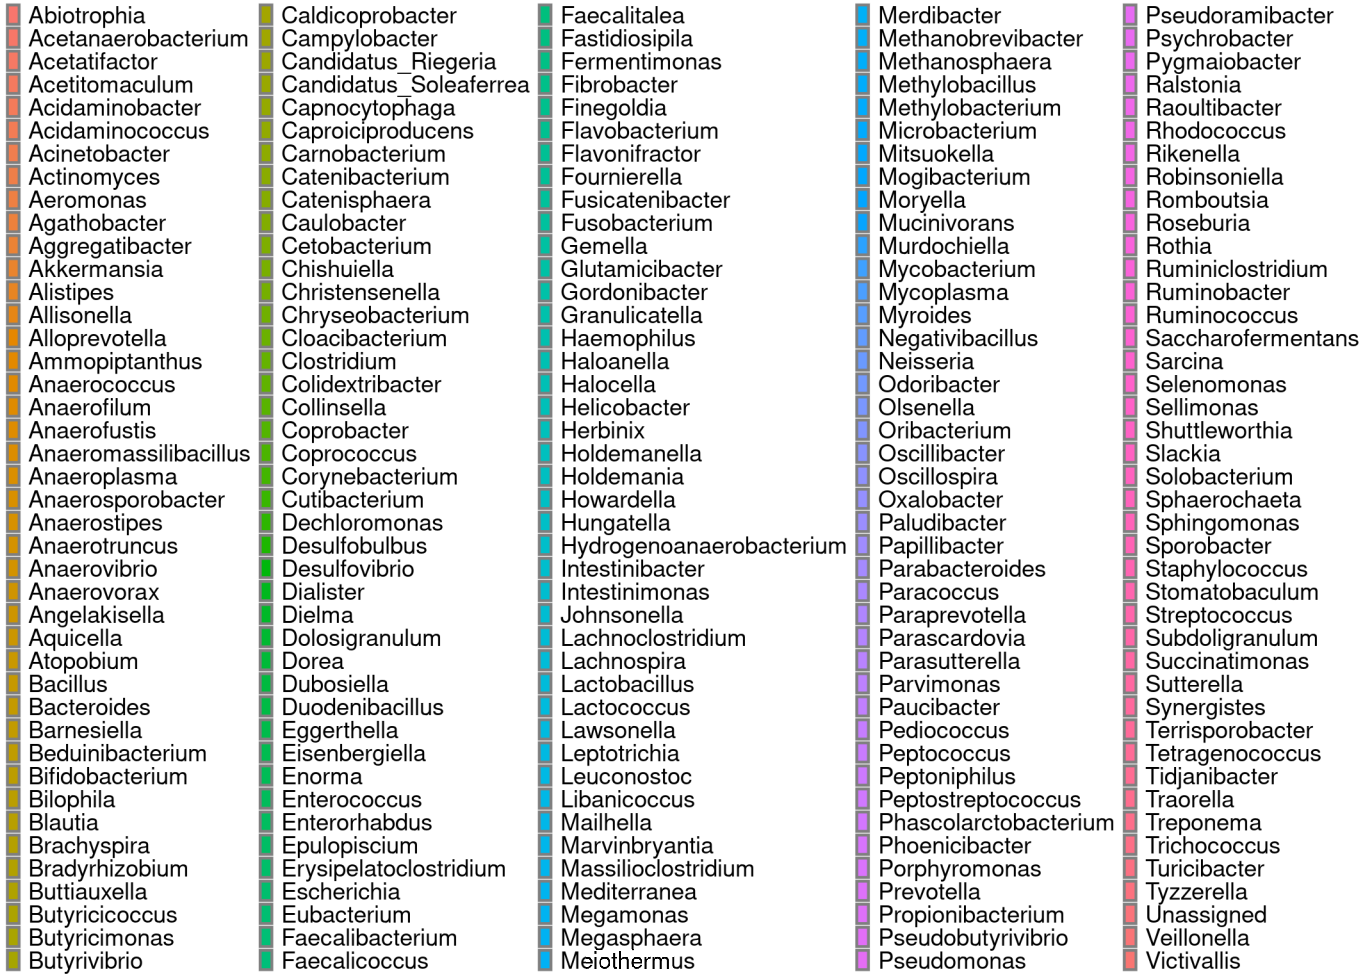
\includegraphics[scale=0.32]{figures/human_gut_abundance_level_g_mgnifyVSgalaxy_legend.png} }}%
  \captionof{figure}[Legend of MGnify human large intestine samples relative abundance plot, comparing MGnify and Galaxy-port at genus rank]{\textbf{Legend of MGnify human large intestine samples relative abundance plot, comparing MGnify and Galaxy-port at genus rank}.} \label{fig:human_gut_abundance_level_g_mgnifyVSgalaxy_legend.png}%
\end{figure}

\begin{figure}[H]
  \centering
  \subfloat{{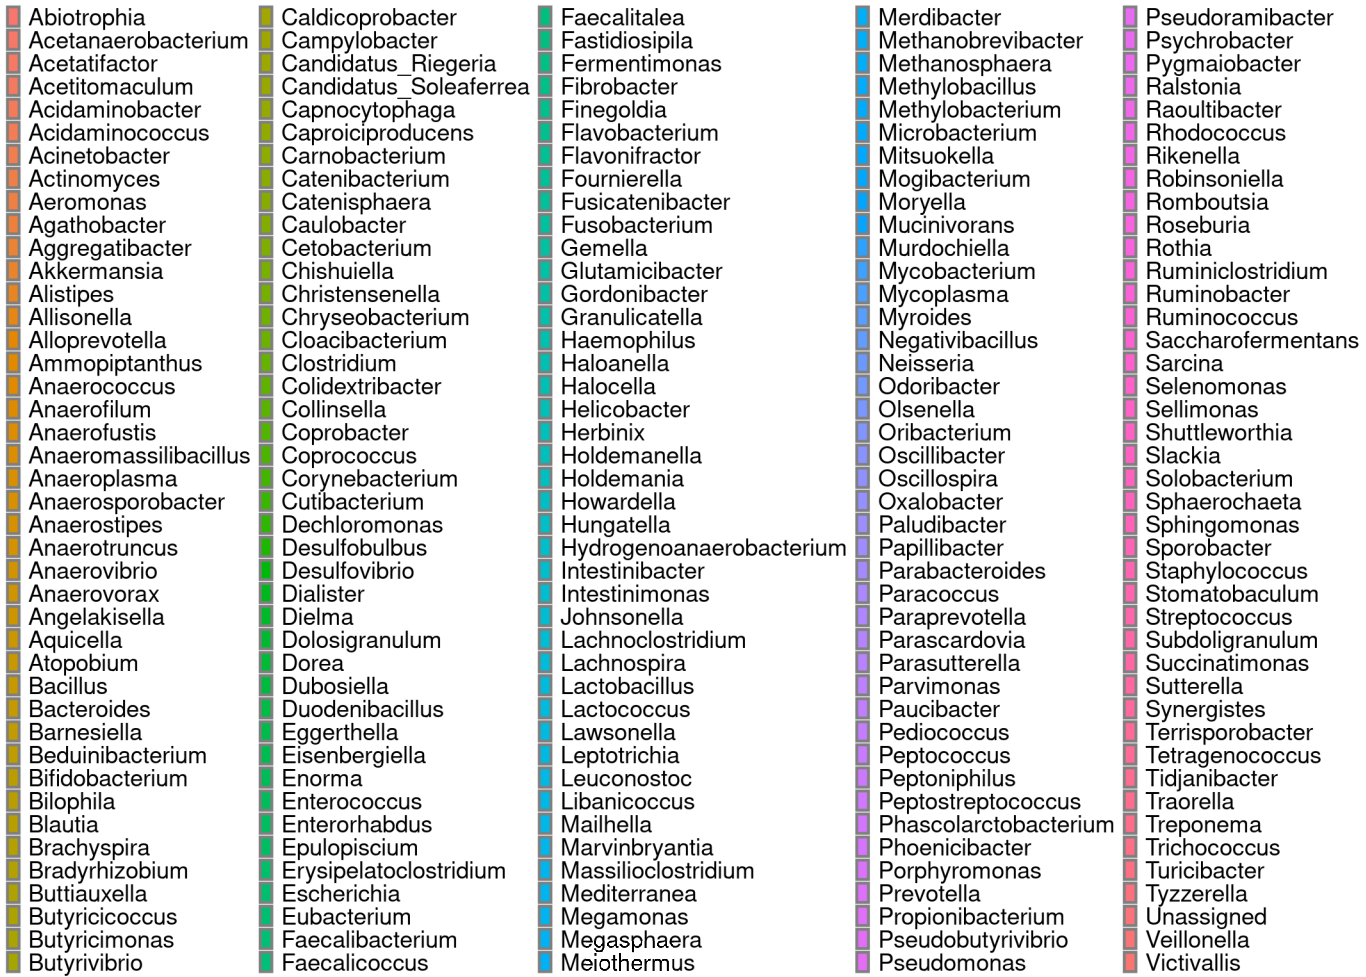
\includegraphics[scale=0.32]{figures/human_gut_abundance_level_g_mgnifyVSKraken_legend.png} }}%
  \captionof{figure}[Legend of MGnify human large intestine samples relative abundance plot, comparing MGnify and Kraken v2 at genus rank]{\textbf{Legend of MGnify human large intestine samples relative abundance plot, comparing MGnify and Kraken v2 at genus rank}.} \label{fig:human_gut_abundance_level_g_mgnifyVSKraken_legend.png}%
\end{figure}

\begin{figure}[H]
  \centering
  \subfloat{{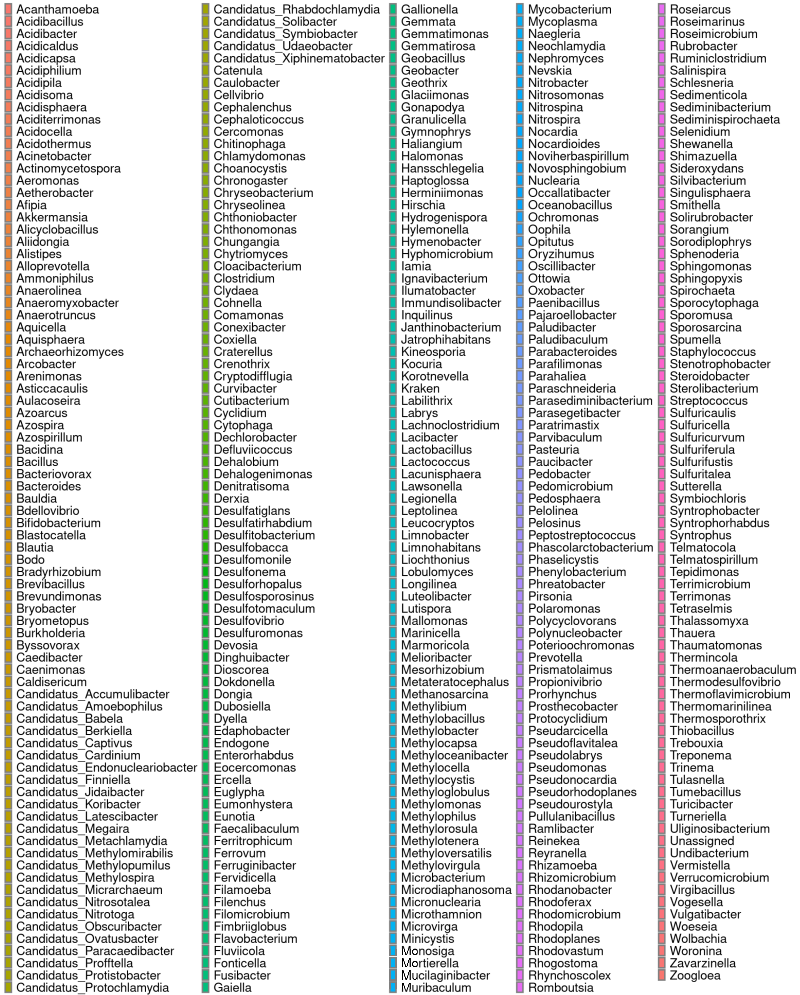
\includegraphics[scale=0.52]{figures/soil_abundance_level_g_mgnifyVSgalaxy_legend.png} }}%
  \captionof{figure}[Legend of MGnify soil samples relative abundance plot, comparing MGnify and Galaxy-port at genus rank]{\textbf{Legend of MGnify soil samples relative abundance plot, comparing MGnify and Galaxy-port at genus rank}.} \label{fig:soil_abundance_level_g_mgnifyVSgalaxy_legend.png}%
\end{figure}

\begin{figure}[H]
  \centering
  \subfloat{{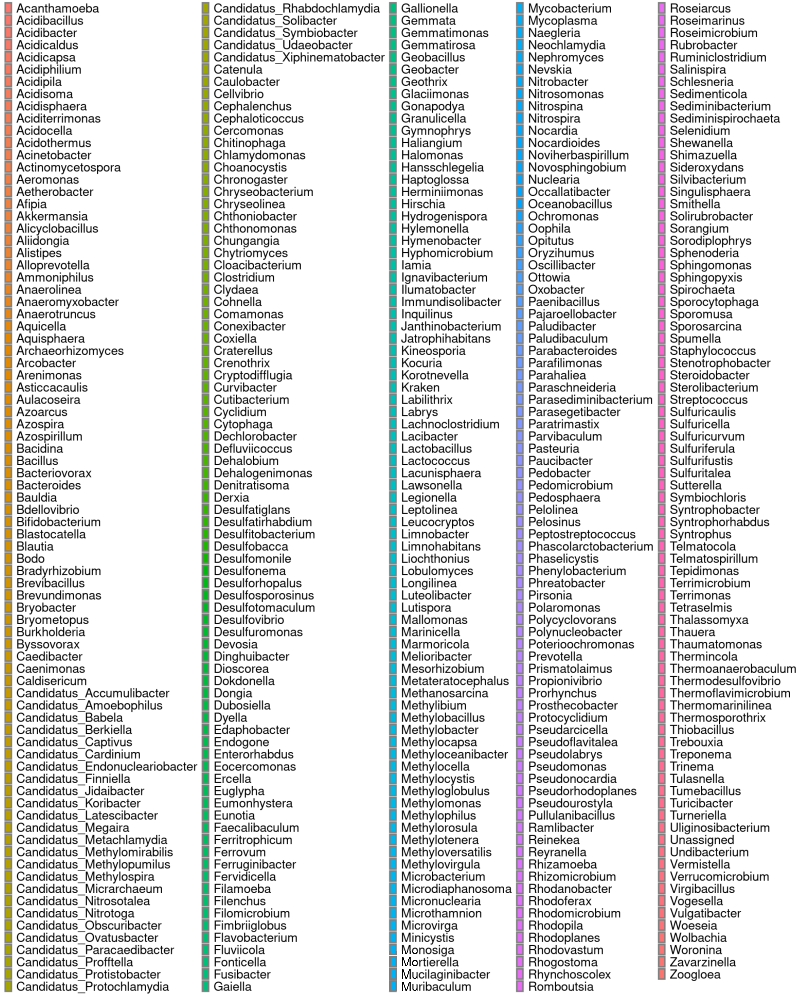
\includegraphics[scale=0.52]{figures/soil_abundance_level_g_mgnifyVSkraken2_legend.png} }}%
  \captionof{figure}[Legend of MGnify soil samples relative abundance plot, comparing MGnify and Kraken v2 at genus rank]{\textbf{Legend of MGnify soil samples relative abundance plot, comparing MGnify and Kraken v2 at genus rank}.} \label{fig:soil_abundance_level_g_mgnifyVSkraken2_legend.png}%
\end{figure}

\begin{figure}[H]
  \centering
  \subfloat{{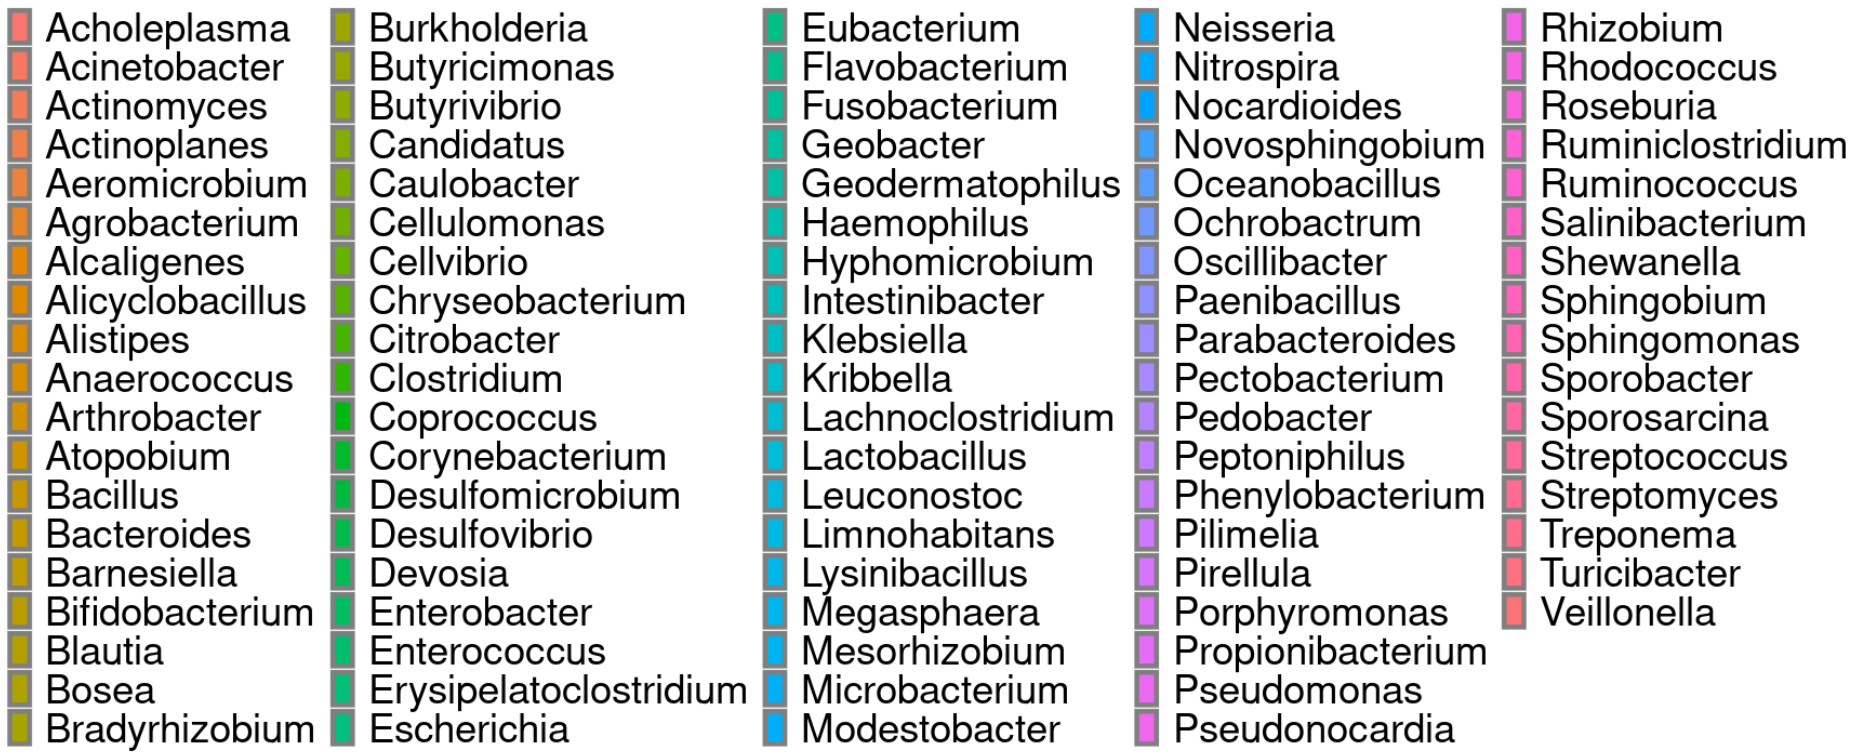
\includegraphics[scale=0.23]{figures/mock_samples_abundance_level_g_legend.png} }}%
  \captionof{figure}[Legend of mock samples relative abundance plot, comparing expected composition, Galaxy-port, and Kraken v2]{\textbf{Legend of mock samples relative abundance plot, comparing expected composition, Galaxy-port, and Kraken v2}.} \label{fig:mock_rel_abundance_level_g_legend}%
\end{figure}

\section{Galaxy workfows}\label{appendix_galaxy_workflows}
\begin{itemize}
    \item rRNA-prediction: \url{https://usegalaxy.eu/u/rz9082/w/rna-prediction}\\
    \item Beta diversity: \url{https://usegalaxy.eu/u/rz9082/w/pairwise-beta-div}
\end{itemize}
\section{Additional software}\label{used_software}
Additional software used during this thesis:
\begin{itemize}
    \item Python v3.7.16, libraries: pandas, seaborn, matplotlib.
    \item R v4.1.2, libraries: ggplot.
\end{itemize}
\section{Results and scripts availability}\label{appendix_results}
All the results obtained and the scripts used for data formatting and visualization during this bachelor thesis are available at: \url{https://drive.google.com/drive/folders/1pgfC_CYVbolskgxhioIXB__449fKtZap}

% If you want a list of your ToDos at the end of the document
% don't forget to remove before submission!
% \input{todo_list}

% \bibliographystyle{unsrt}
% \bibliography{bib/webpages,bib/articles}
% bibliography is not in the table of contents per default, add it manually
% enable the \renewcommand for german header
\listoftables
\listoffigures
% 
\printbibliography
\renewcommand{\bibname}{Bibliography}
\addcontentsline{toc}{chapter}{Bibliography}
\newpage
\thispagestyle{empty}
\mbox{}


\end{document}